\chapter{Задача слежения для системы с астатизмом первого порядка
(ПИ-регулятор)}
Рассмотрим замкнутую систему с пропорционально-интегральным регулятором (Схема задана на рисунке
\hyperref[fig:sim4]{\ref{fig:sim4}}). Зададимся следующими парами параметрами $k_p$ и $k_i$:
\begin{itemize}
    \item $k_p = 5$, $k_p = 10$, $k_p = 25$
    \item $k_i = 0.1$, $k_i = 1$, $k_i = 5$
\end{itemize}
\section{Режим движения с постоянной скоростью $g(t) = Vt$}
Выполним моделирование:
\begin{figure}[H]
    \centering
    \begin{minipage}{0.45\textwidth}
        \centering
        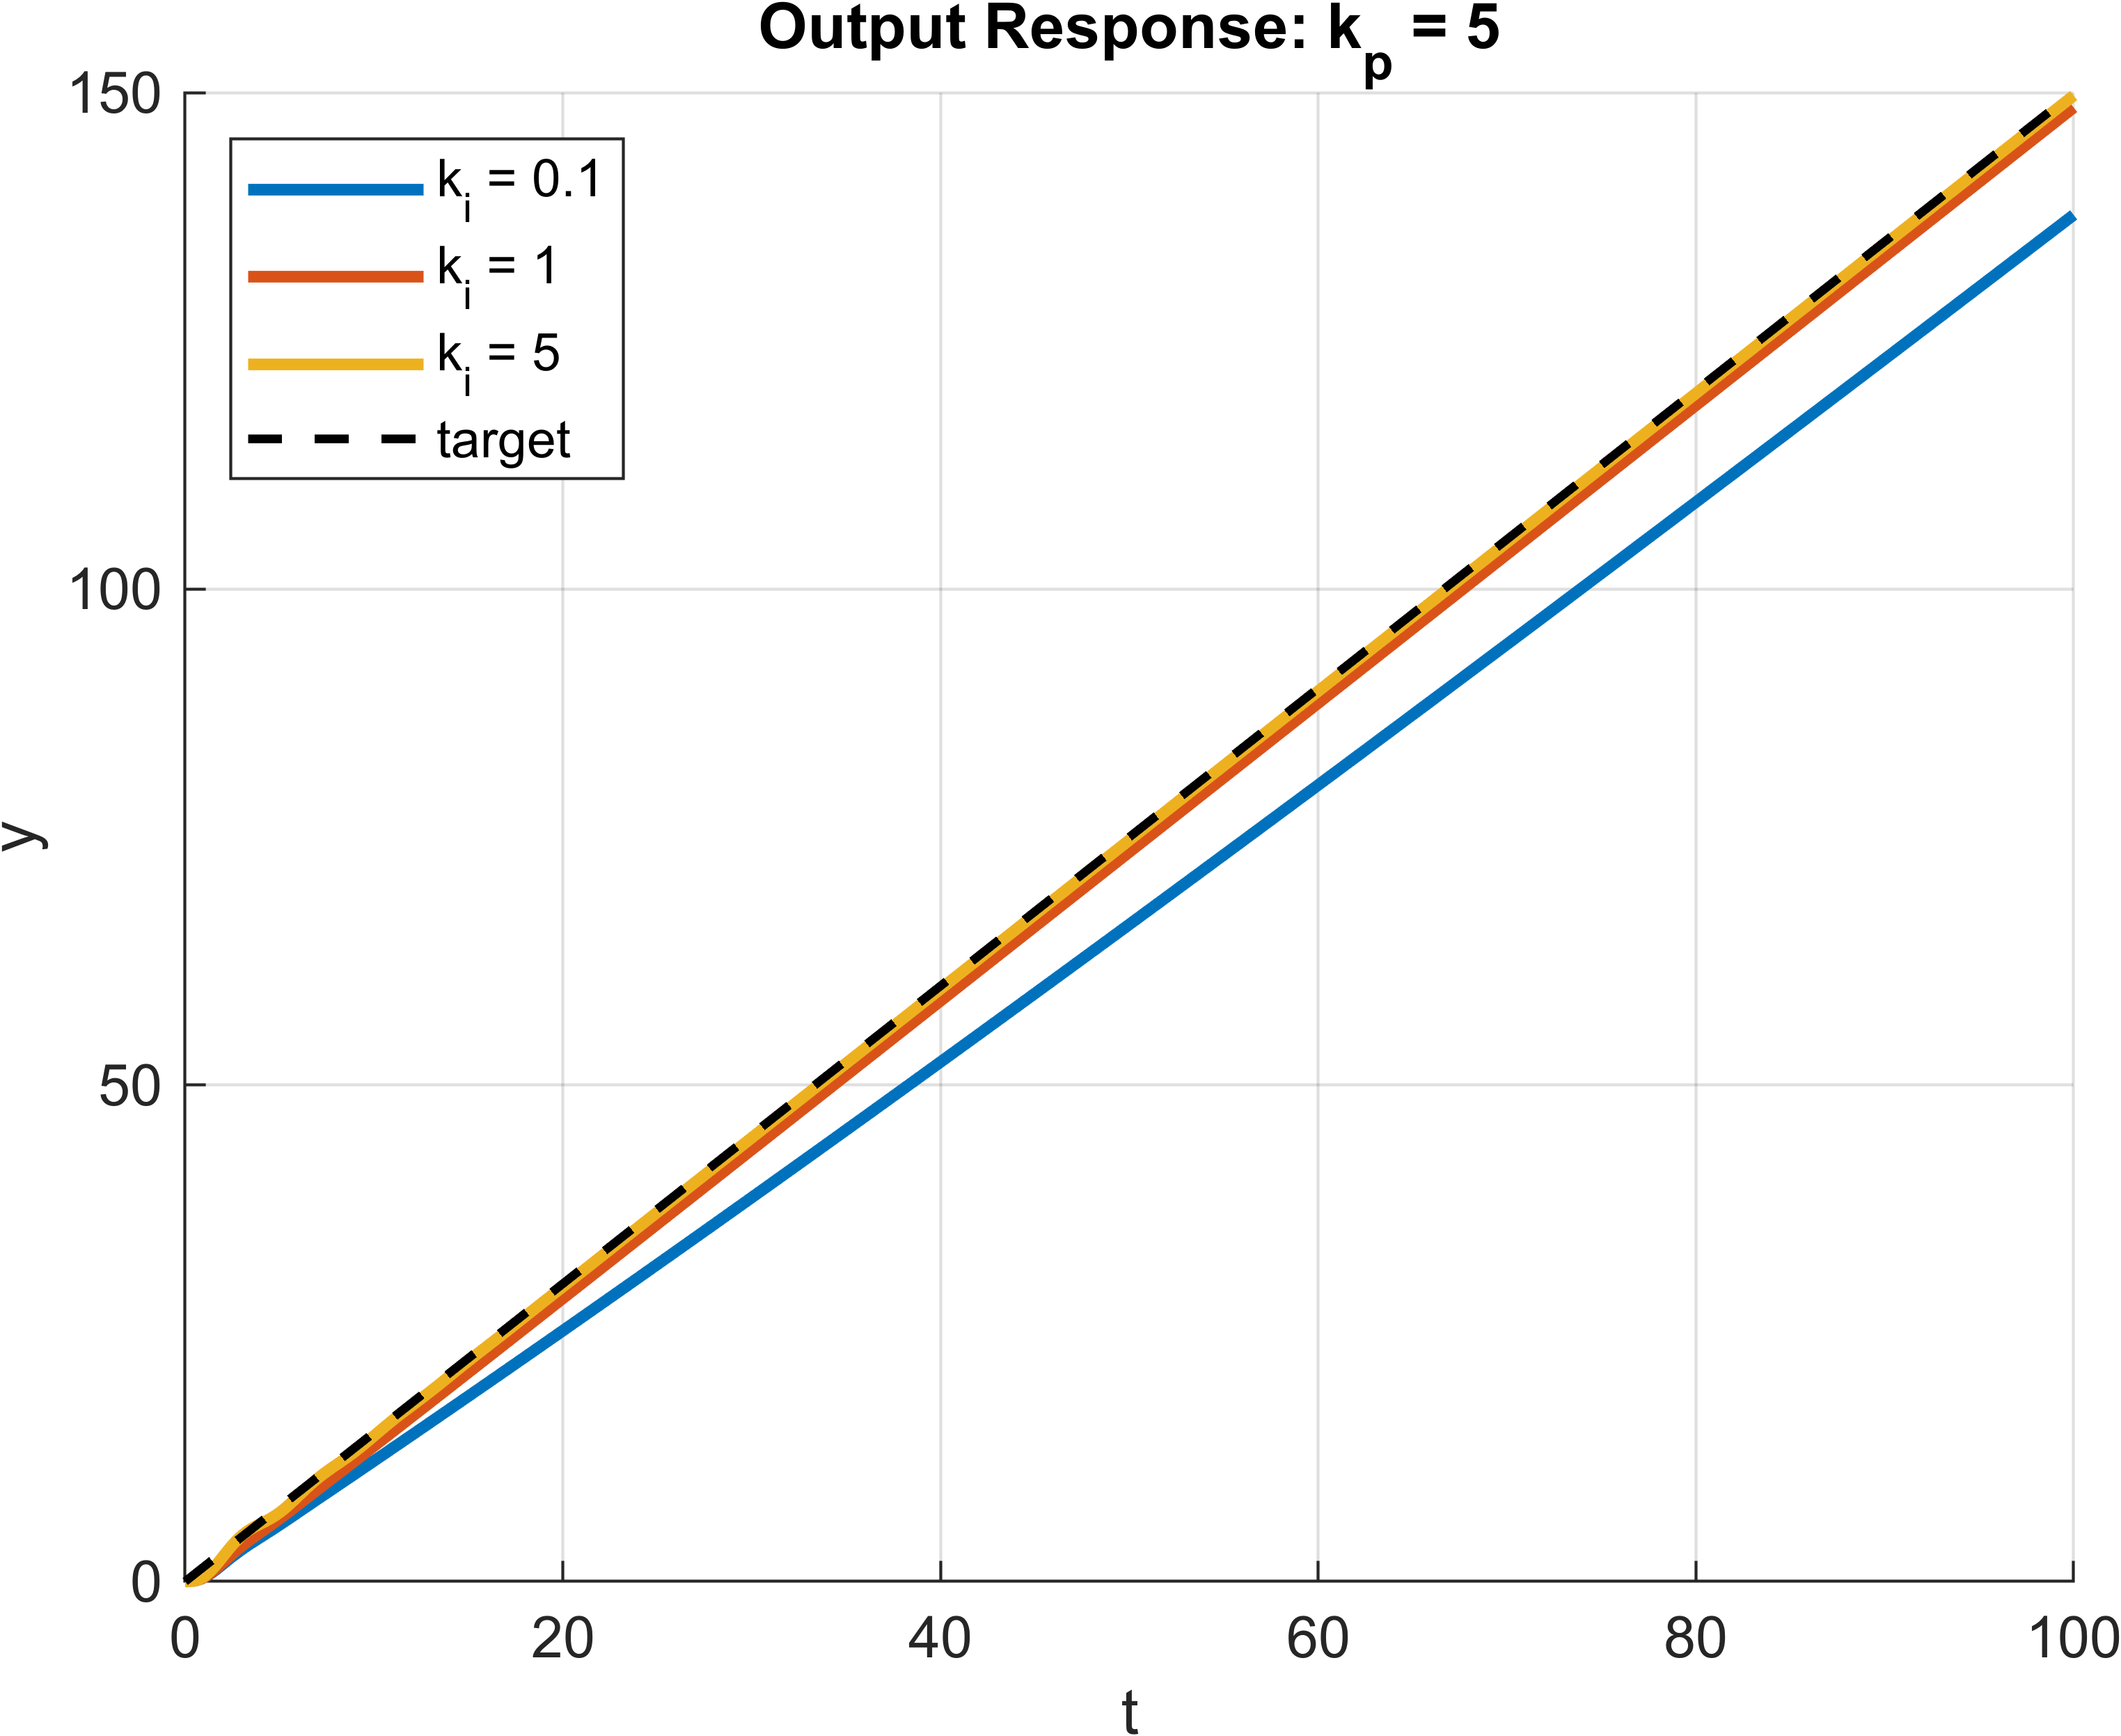
\includegraphics[width=1\textwidth, trim={1cm 0cm 1cm 0cm}]{../images/input_2_kp_5_output.png}
    \end{minipage}
    \hfill
    \begin{minipage}{0.45\textwidth}
        \centering
        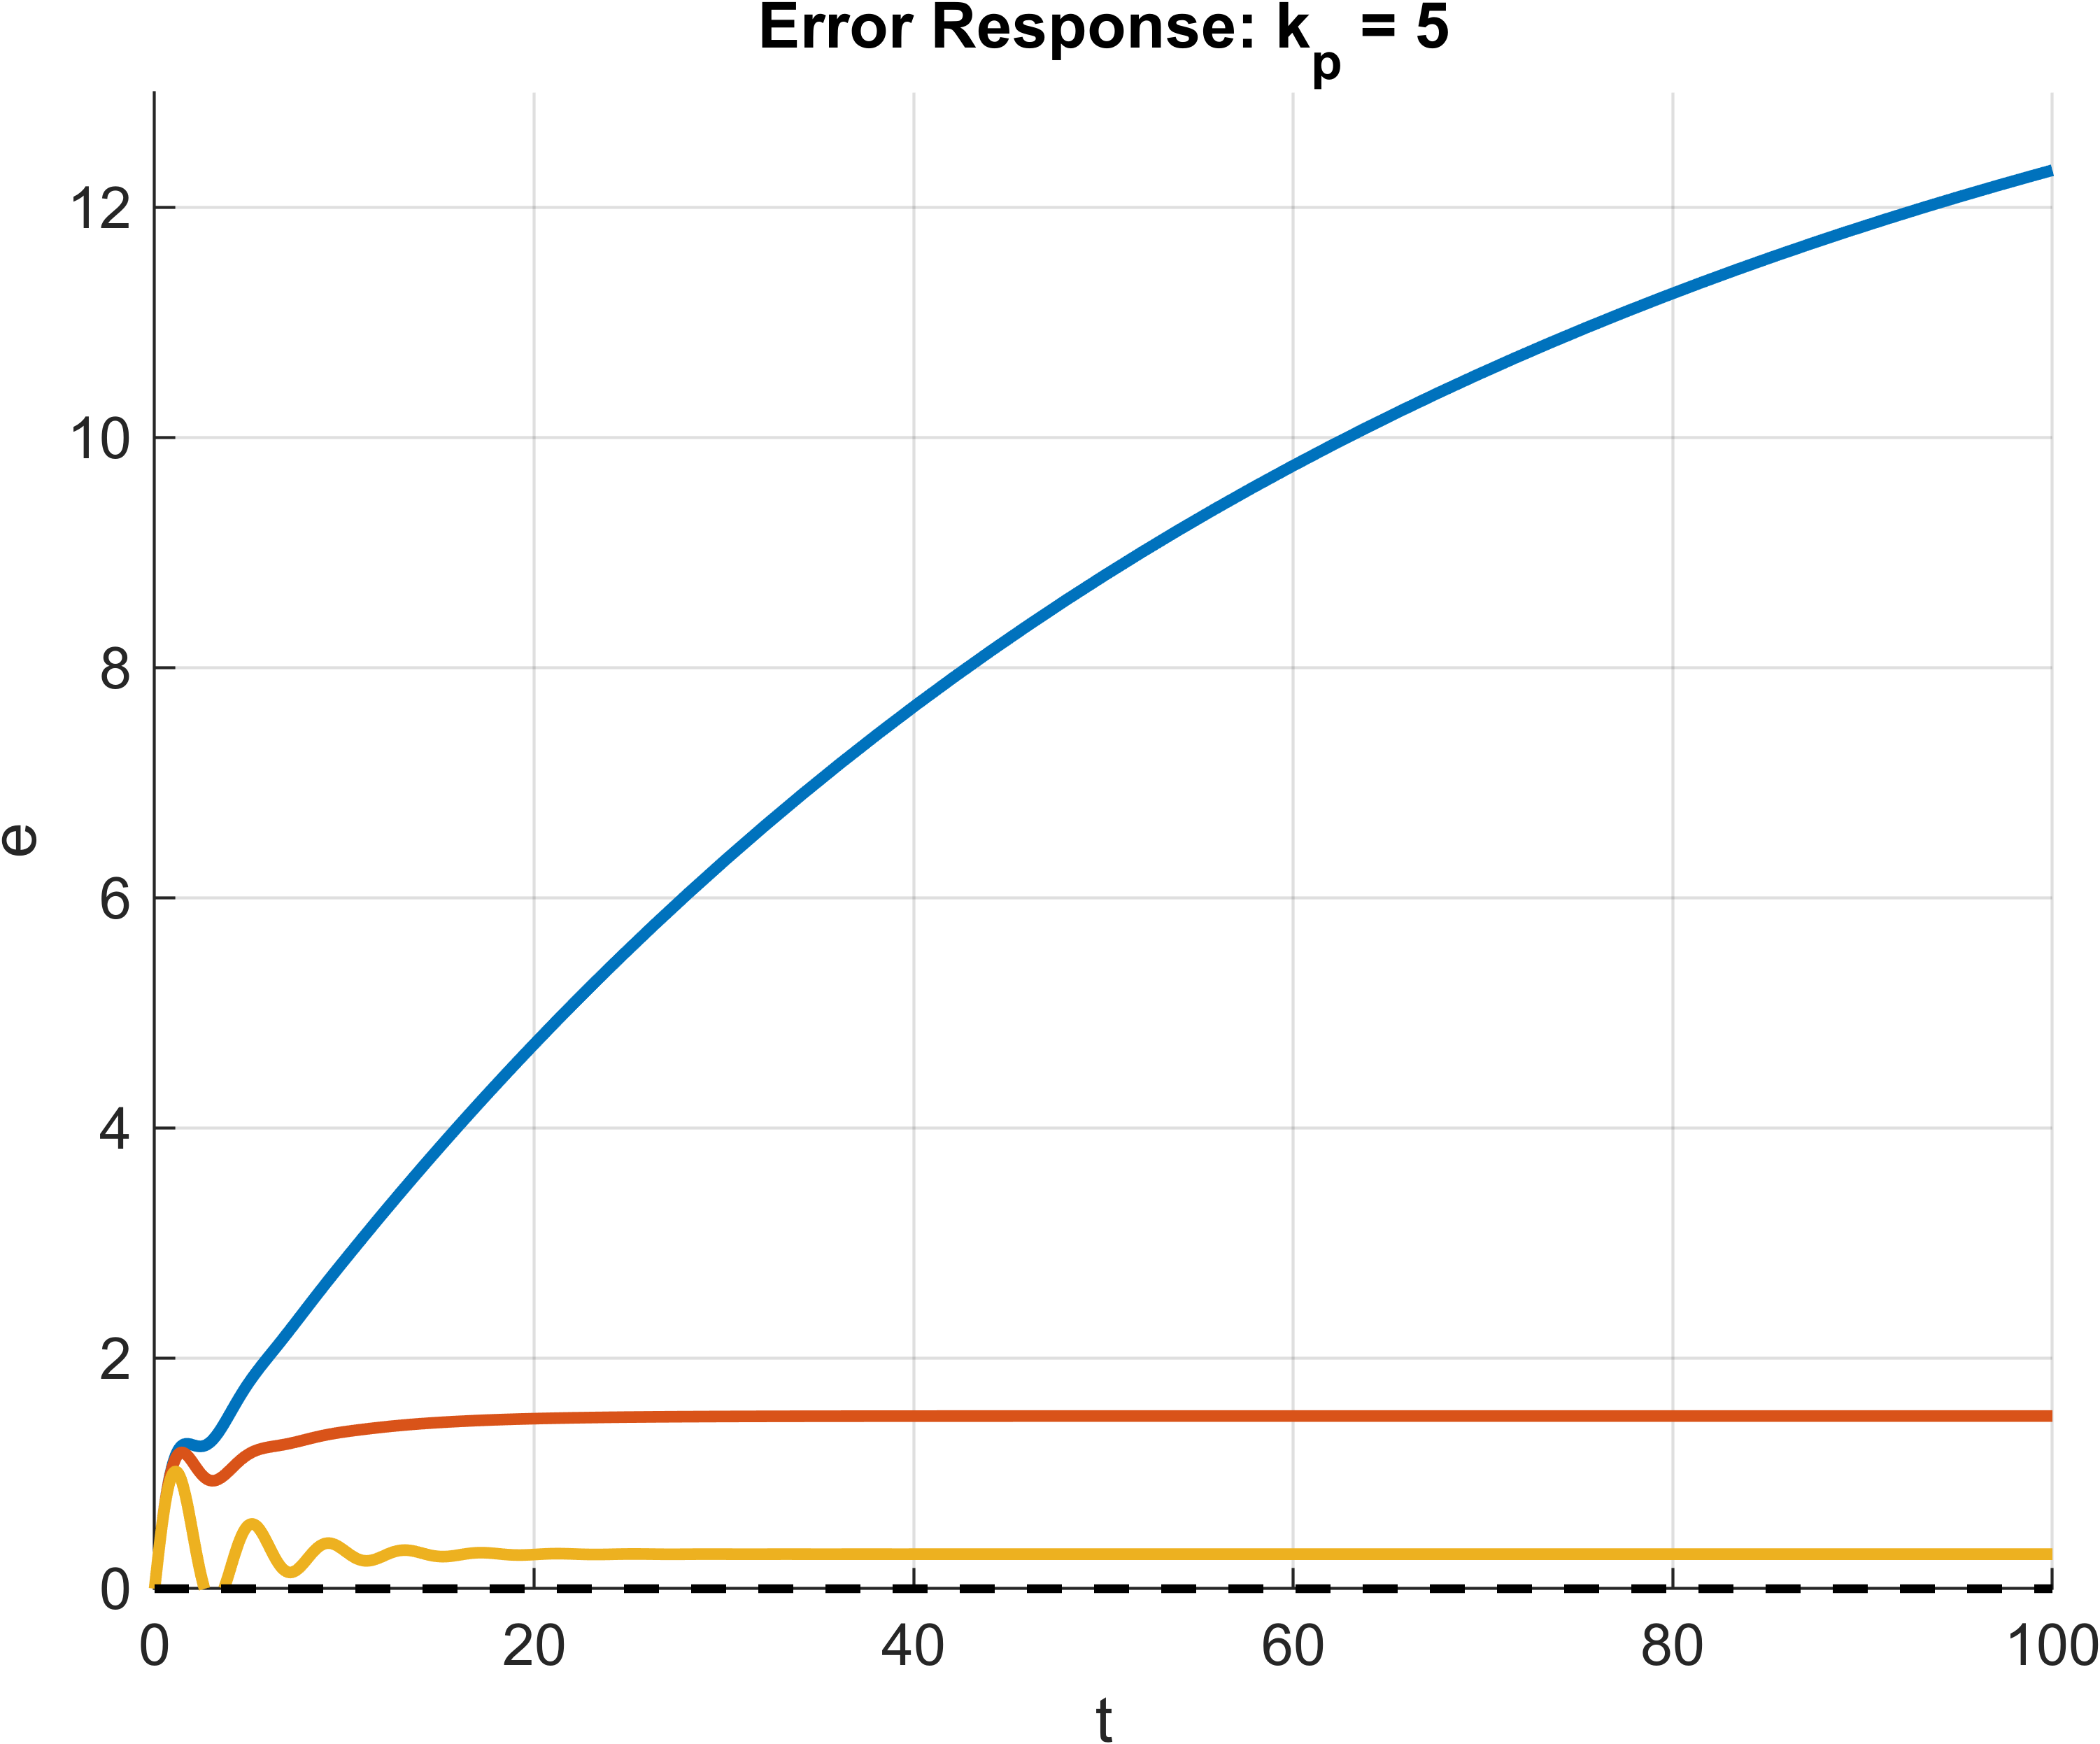
\includegraphics[width=1\textwidth, trim={1cm 0cm 1cm 0cm}]{../images/input_2_kp_5_error.png}
    \end{minipage}
    \caption{Графики $y(t)$ и $e(t)$ при $g(t) = 1.5t$ и $k_p = 5$}
\end{figure}
\begin{figure}[H]
    \centering
    \begin{minipage}{0.45\textwidth}
        \centering
        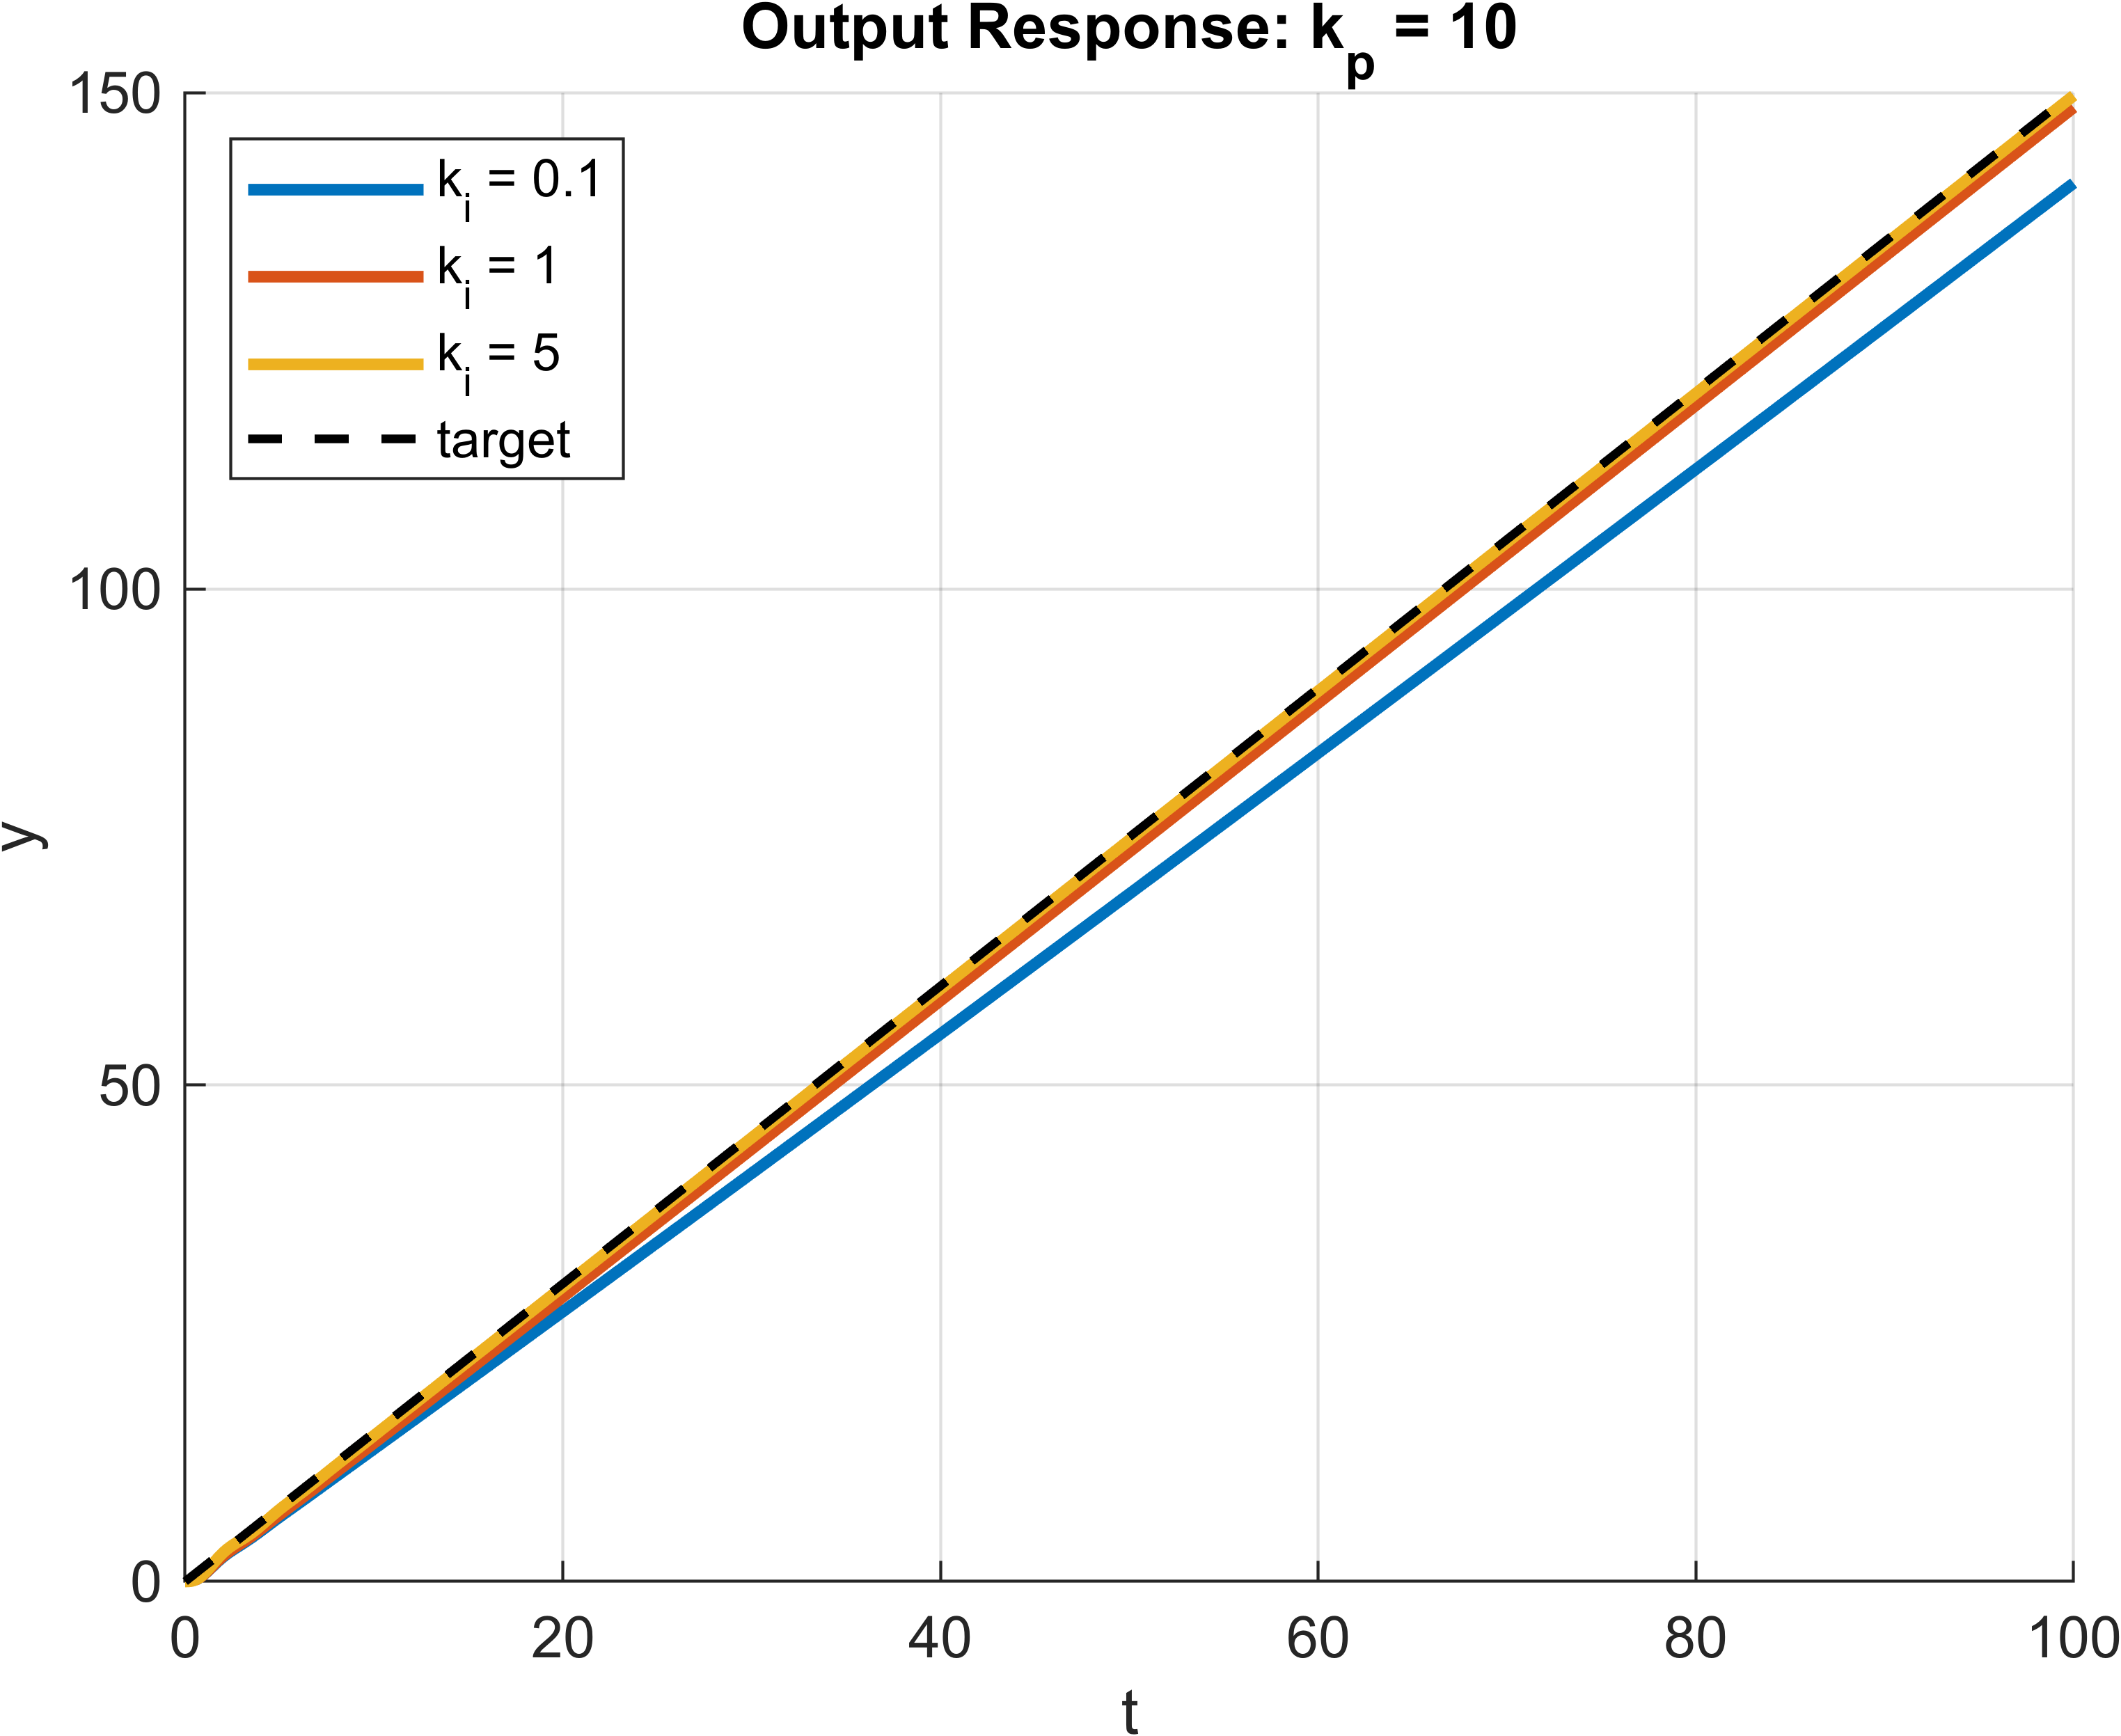
\includegraphics[width=1\textwidth, trim={1cm 0cm 1cm 0cm}]{../images/input_2_kp_10_output.png}
    \end{minipage}
    \hfill
    \begin{minipage}{0.45\textwidth}
        \centering
        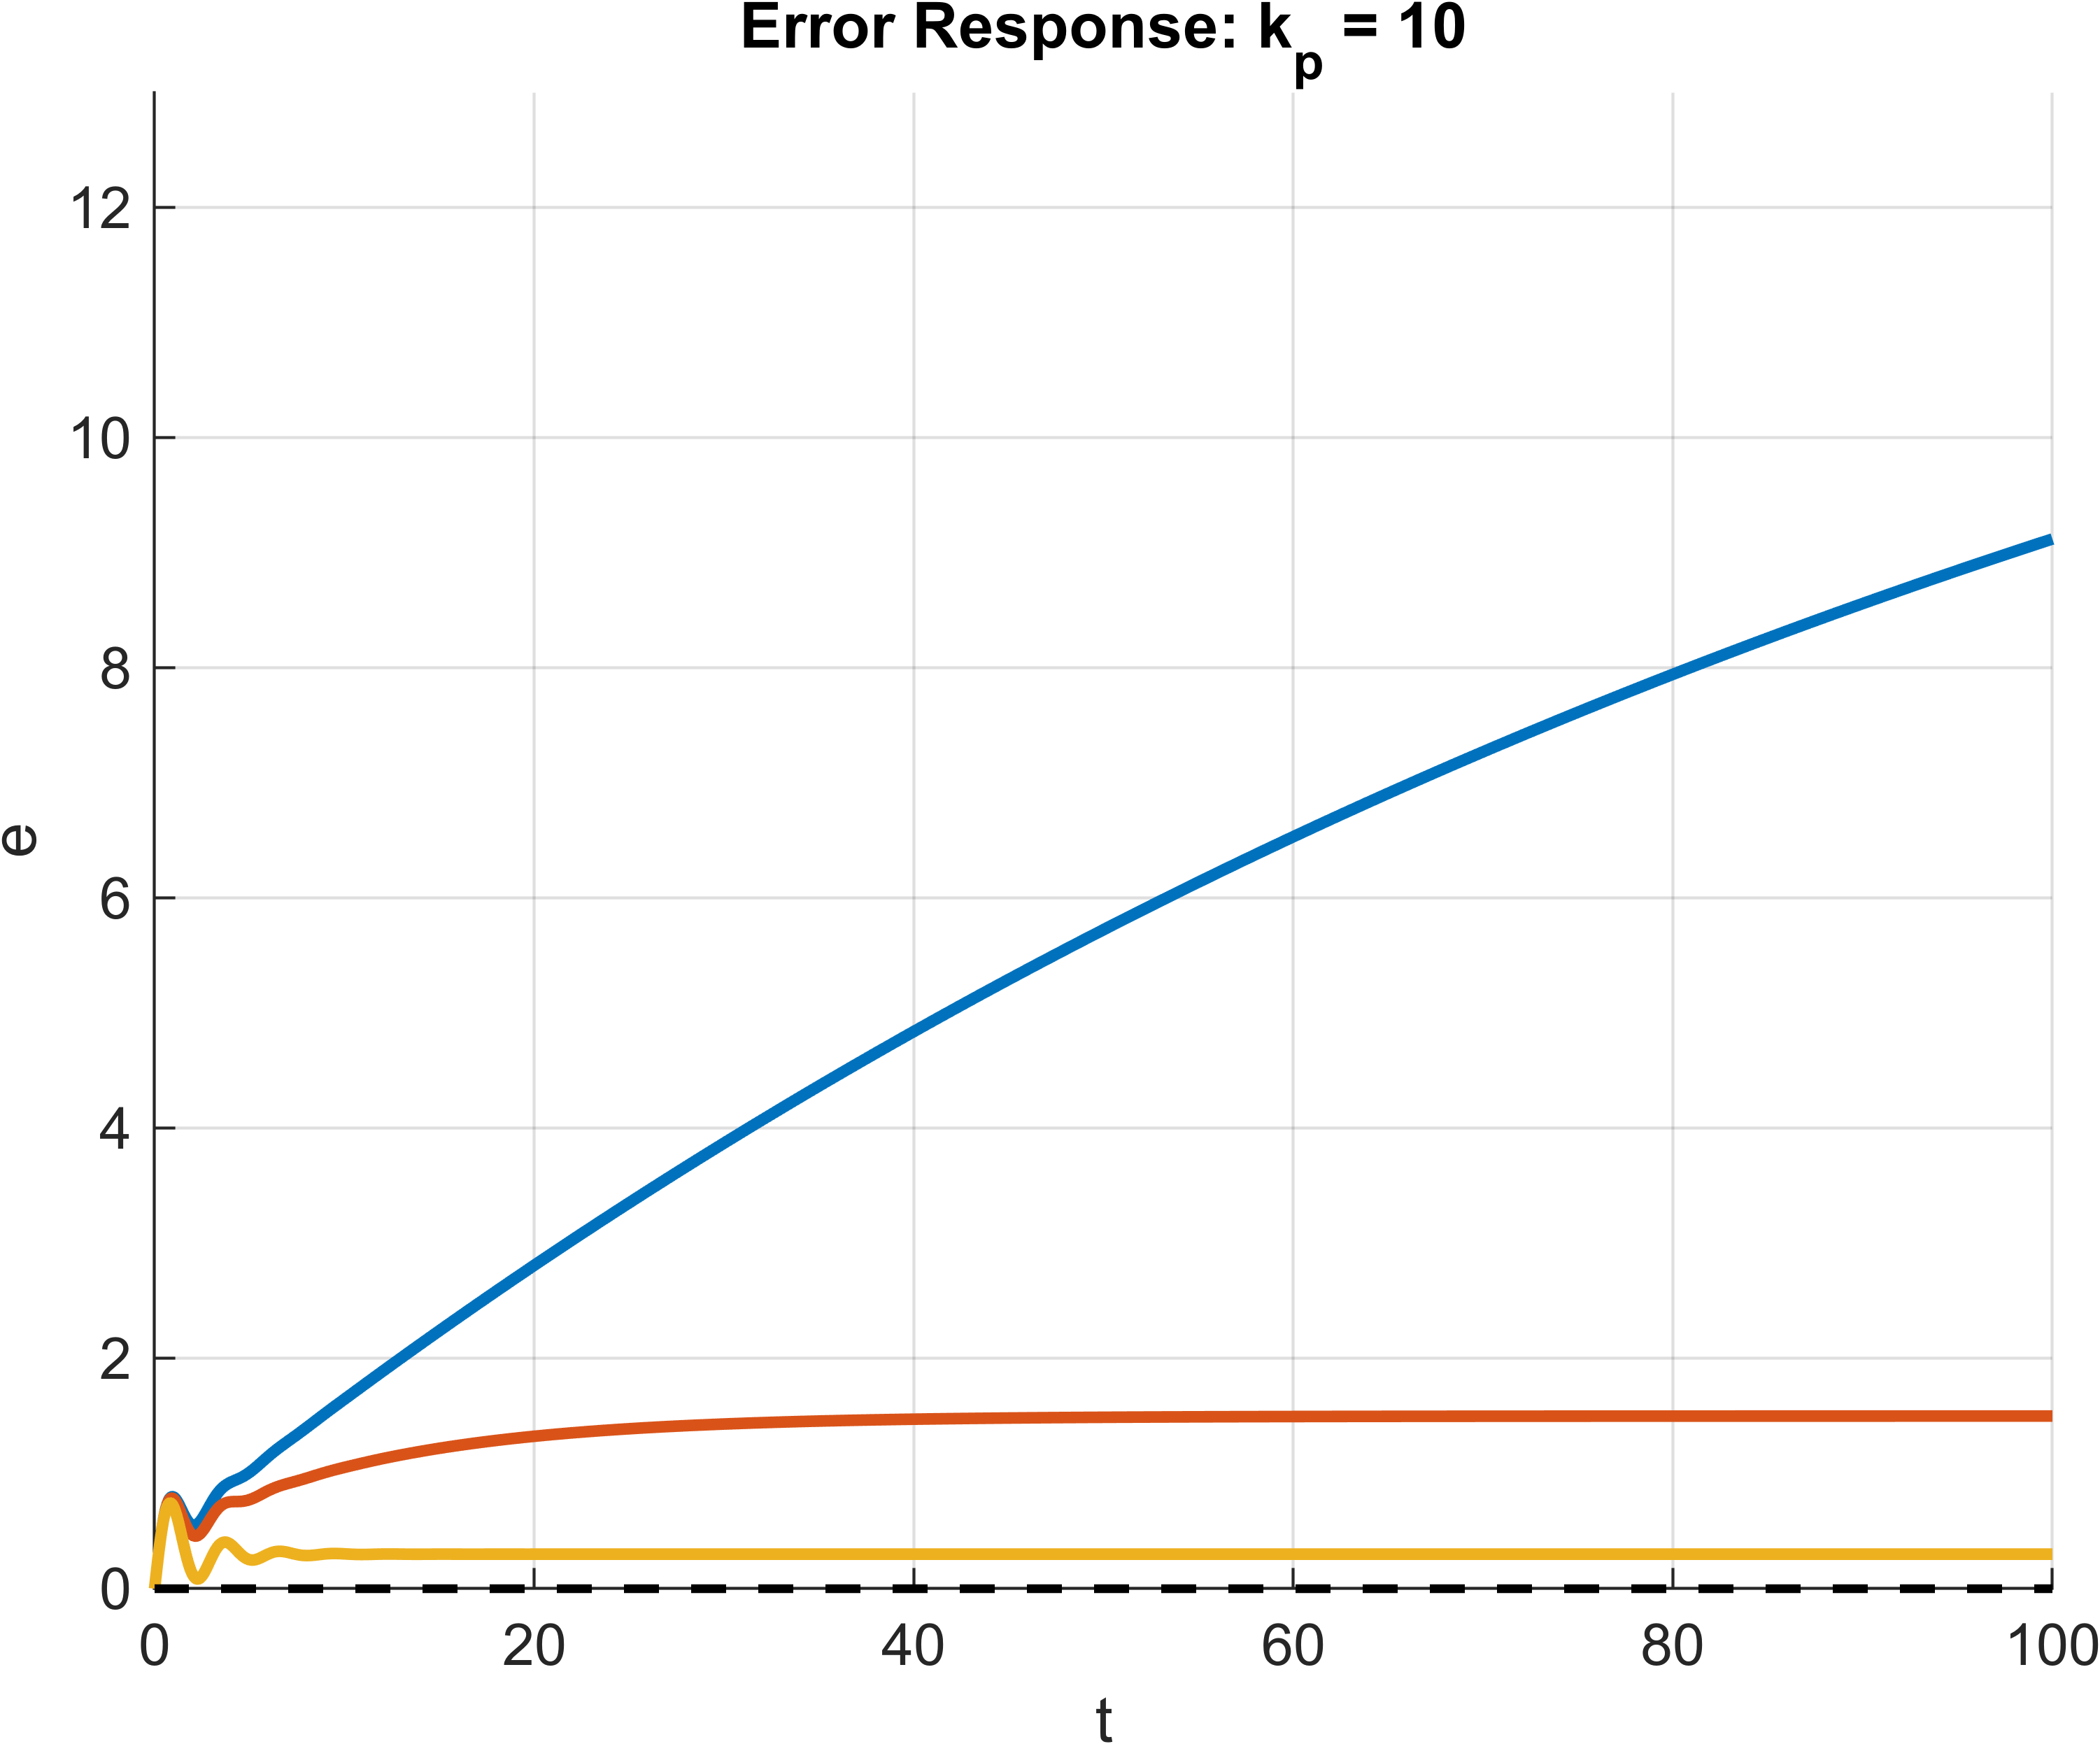
\includegraphics[width=1\textwidth, trim={1cm 0cm 1cm 0cm}]{../images/input_2_kp_10_error.png}
    \end{minipage}
    \caption{Графики $y(t)$ и $e(t)$ при $g(t) = 1.5t$ и $k_p = 10$}
\end{figure}
\begin{figure}[H]
    \centering
    \begin{minipage}{0.45\textwidth}
        \centering
        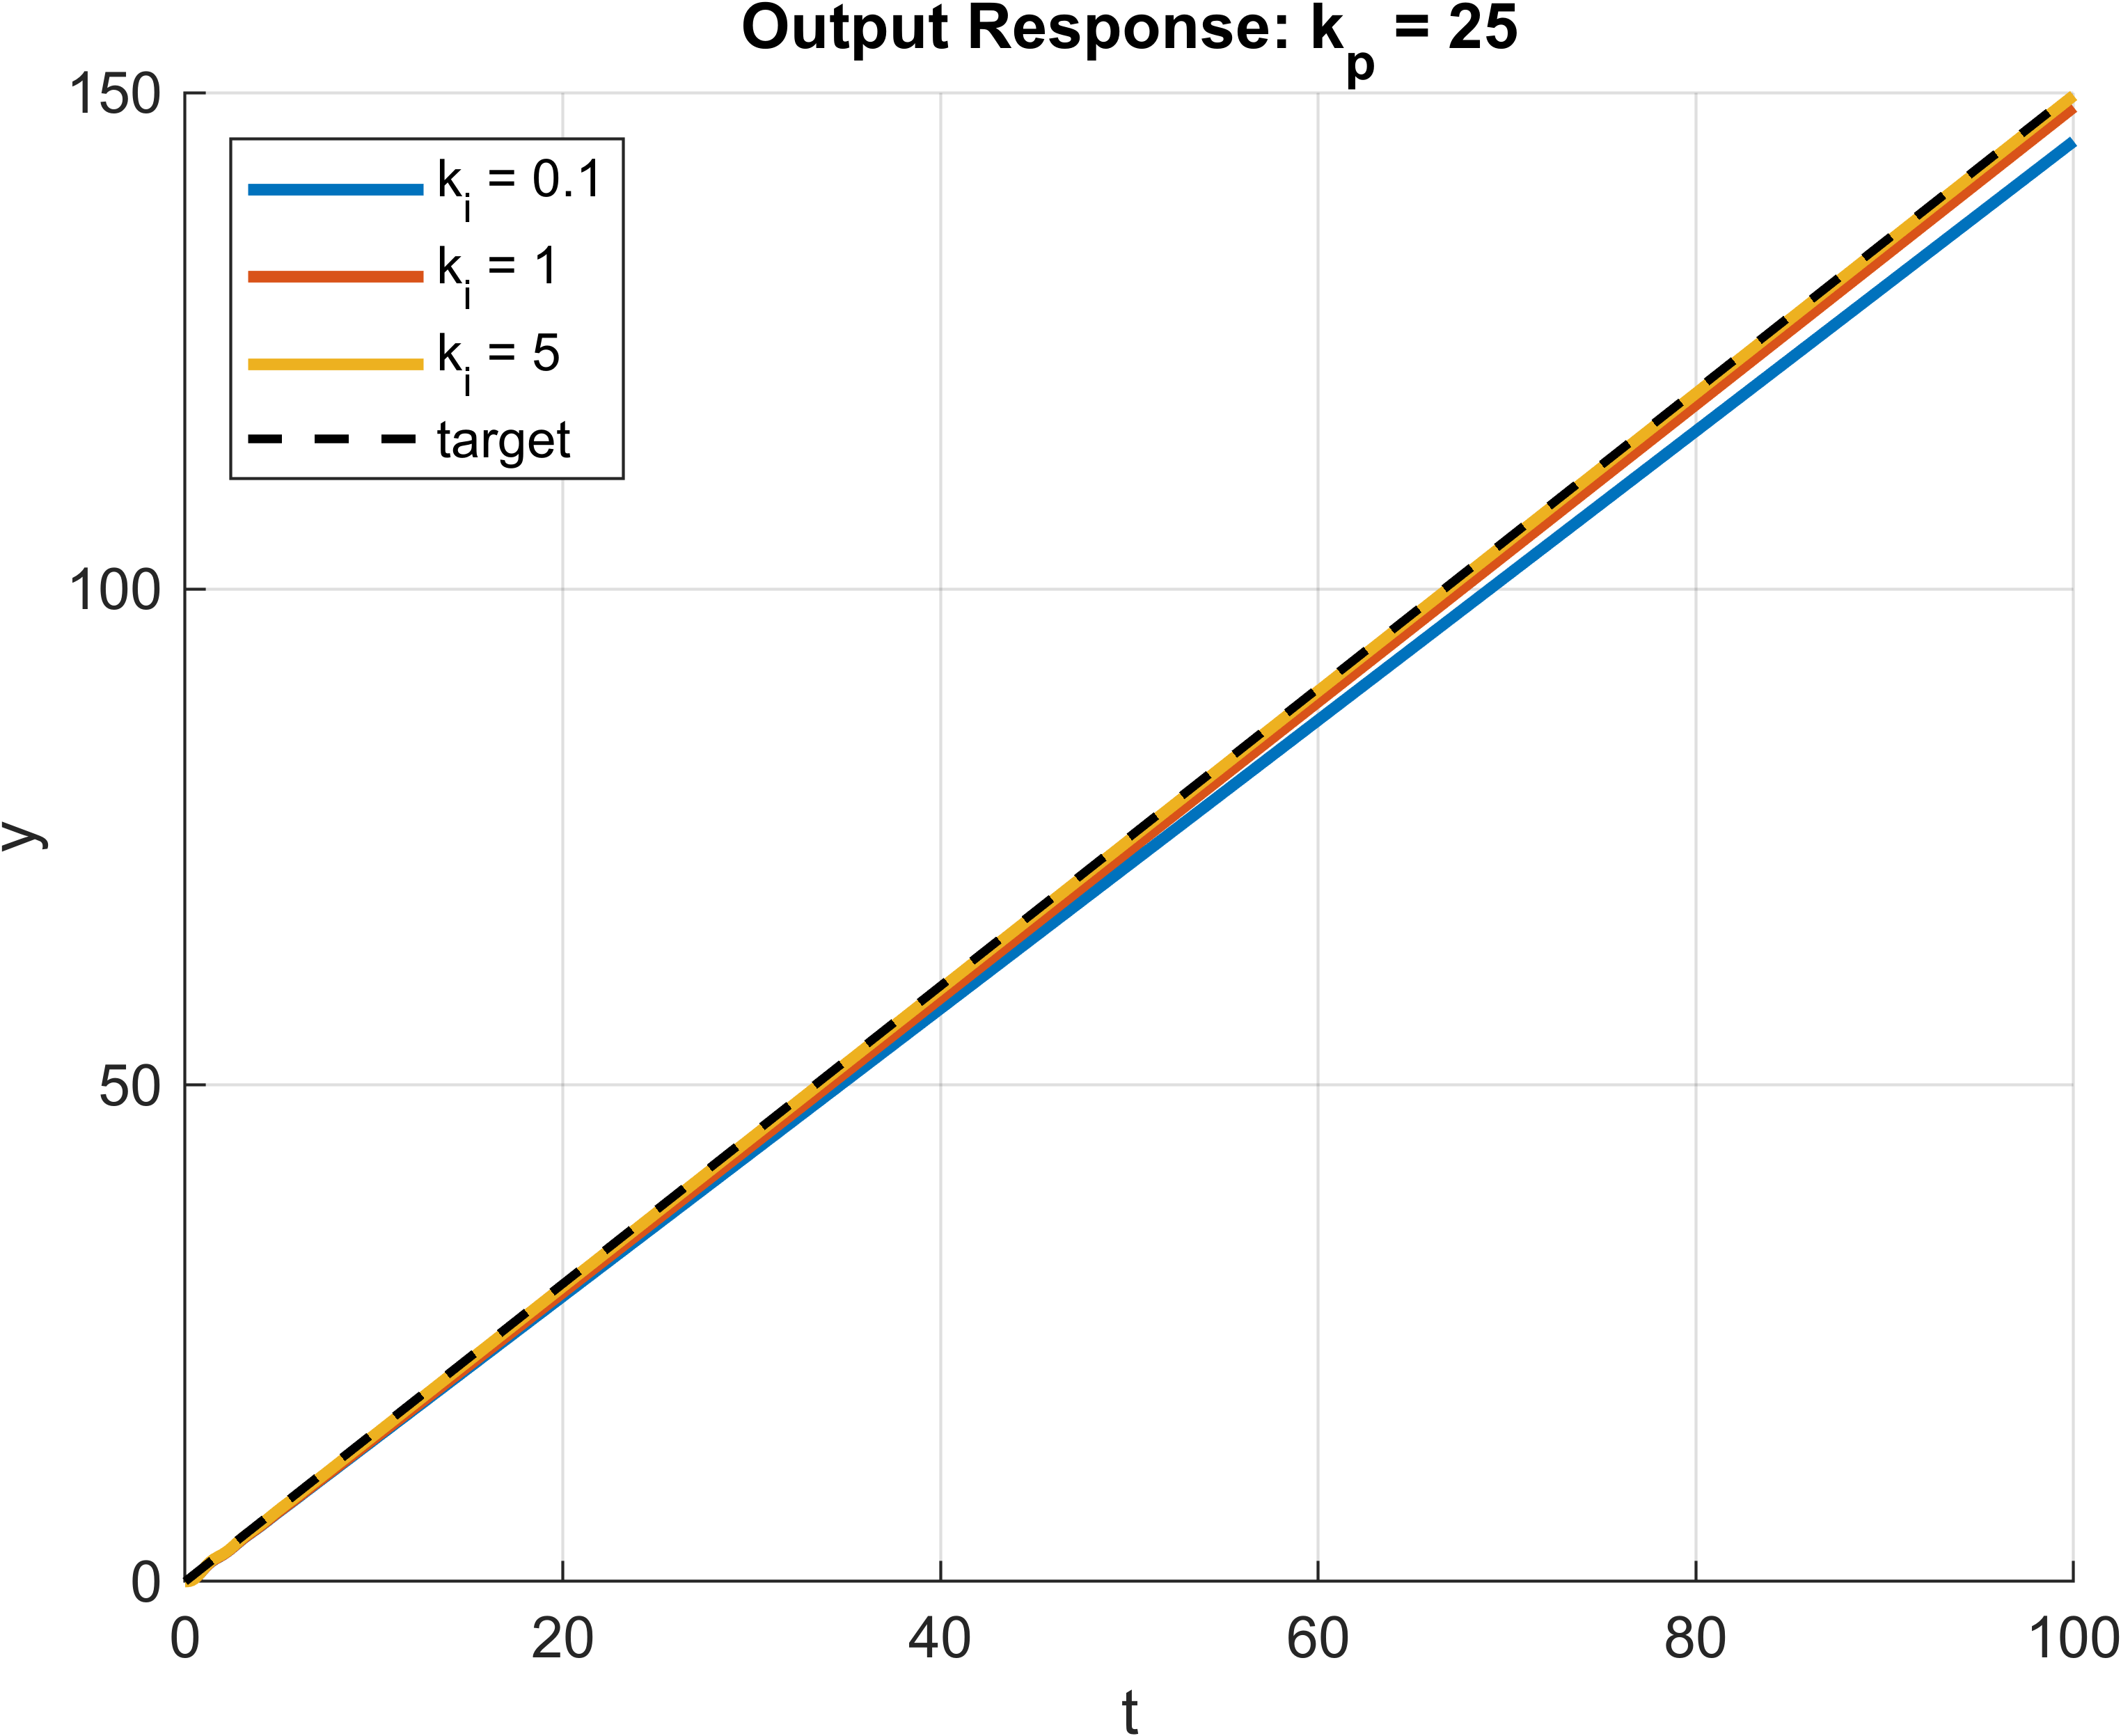
\includegraphics[width=1\textwidth, trim={1cm 0cm 1cm 0cm}]{../images/input_2_kp_25_output.png}
    \end{minipage}
    \hfill
    \begin{minipage}{0.45\textwidth}
        \centering
        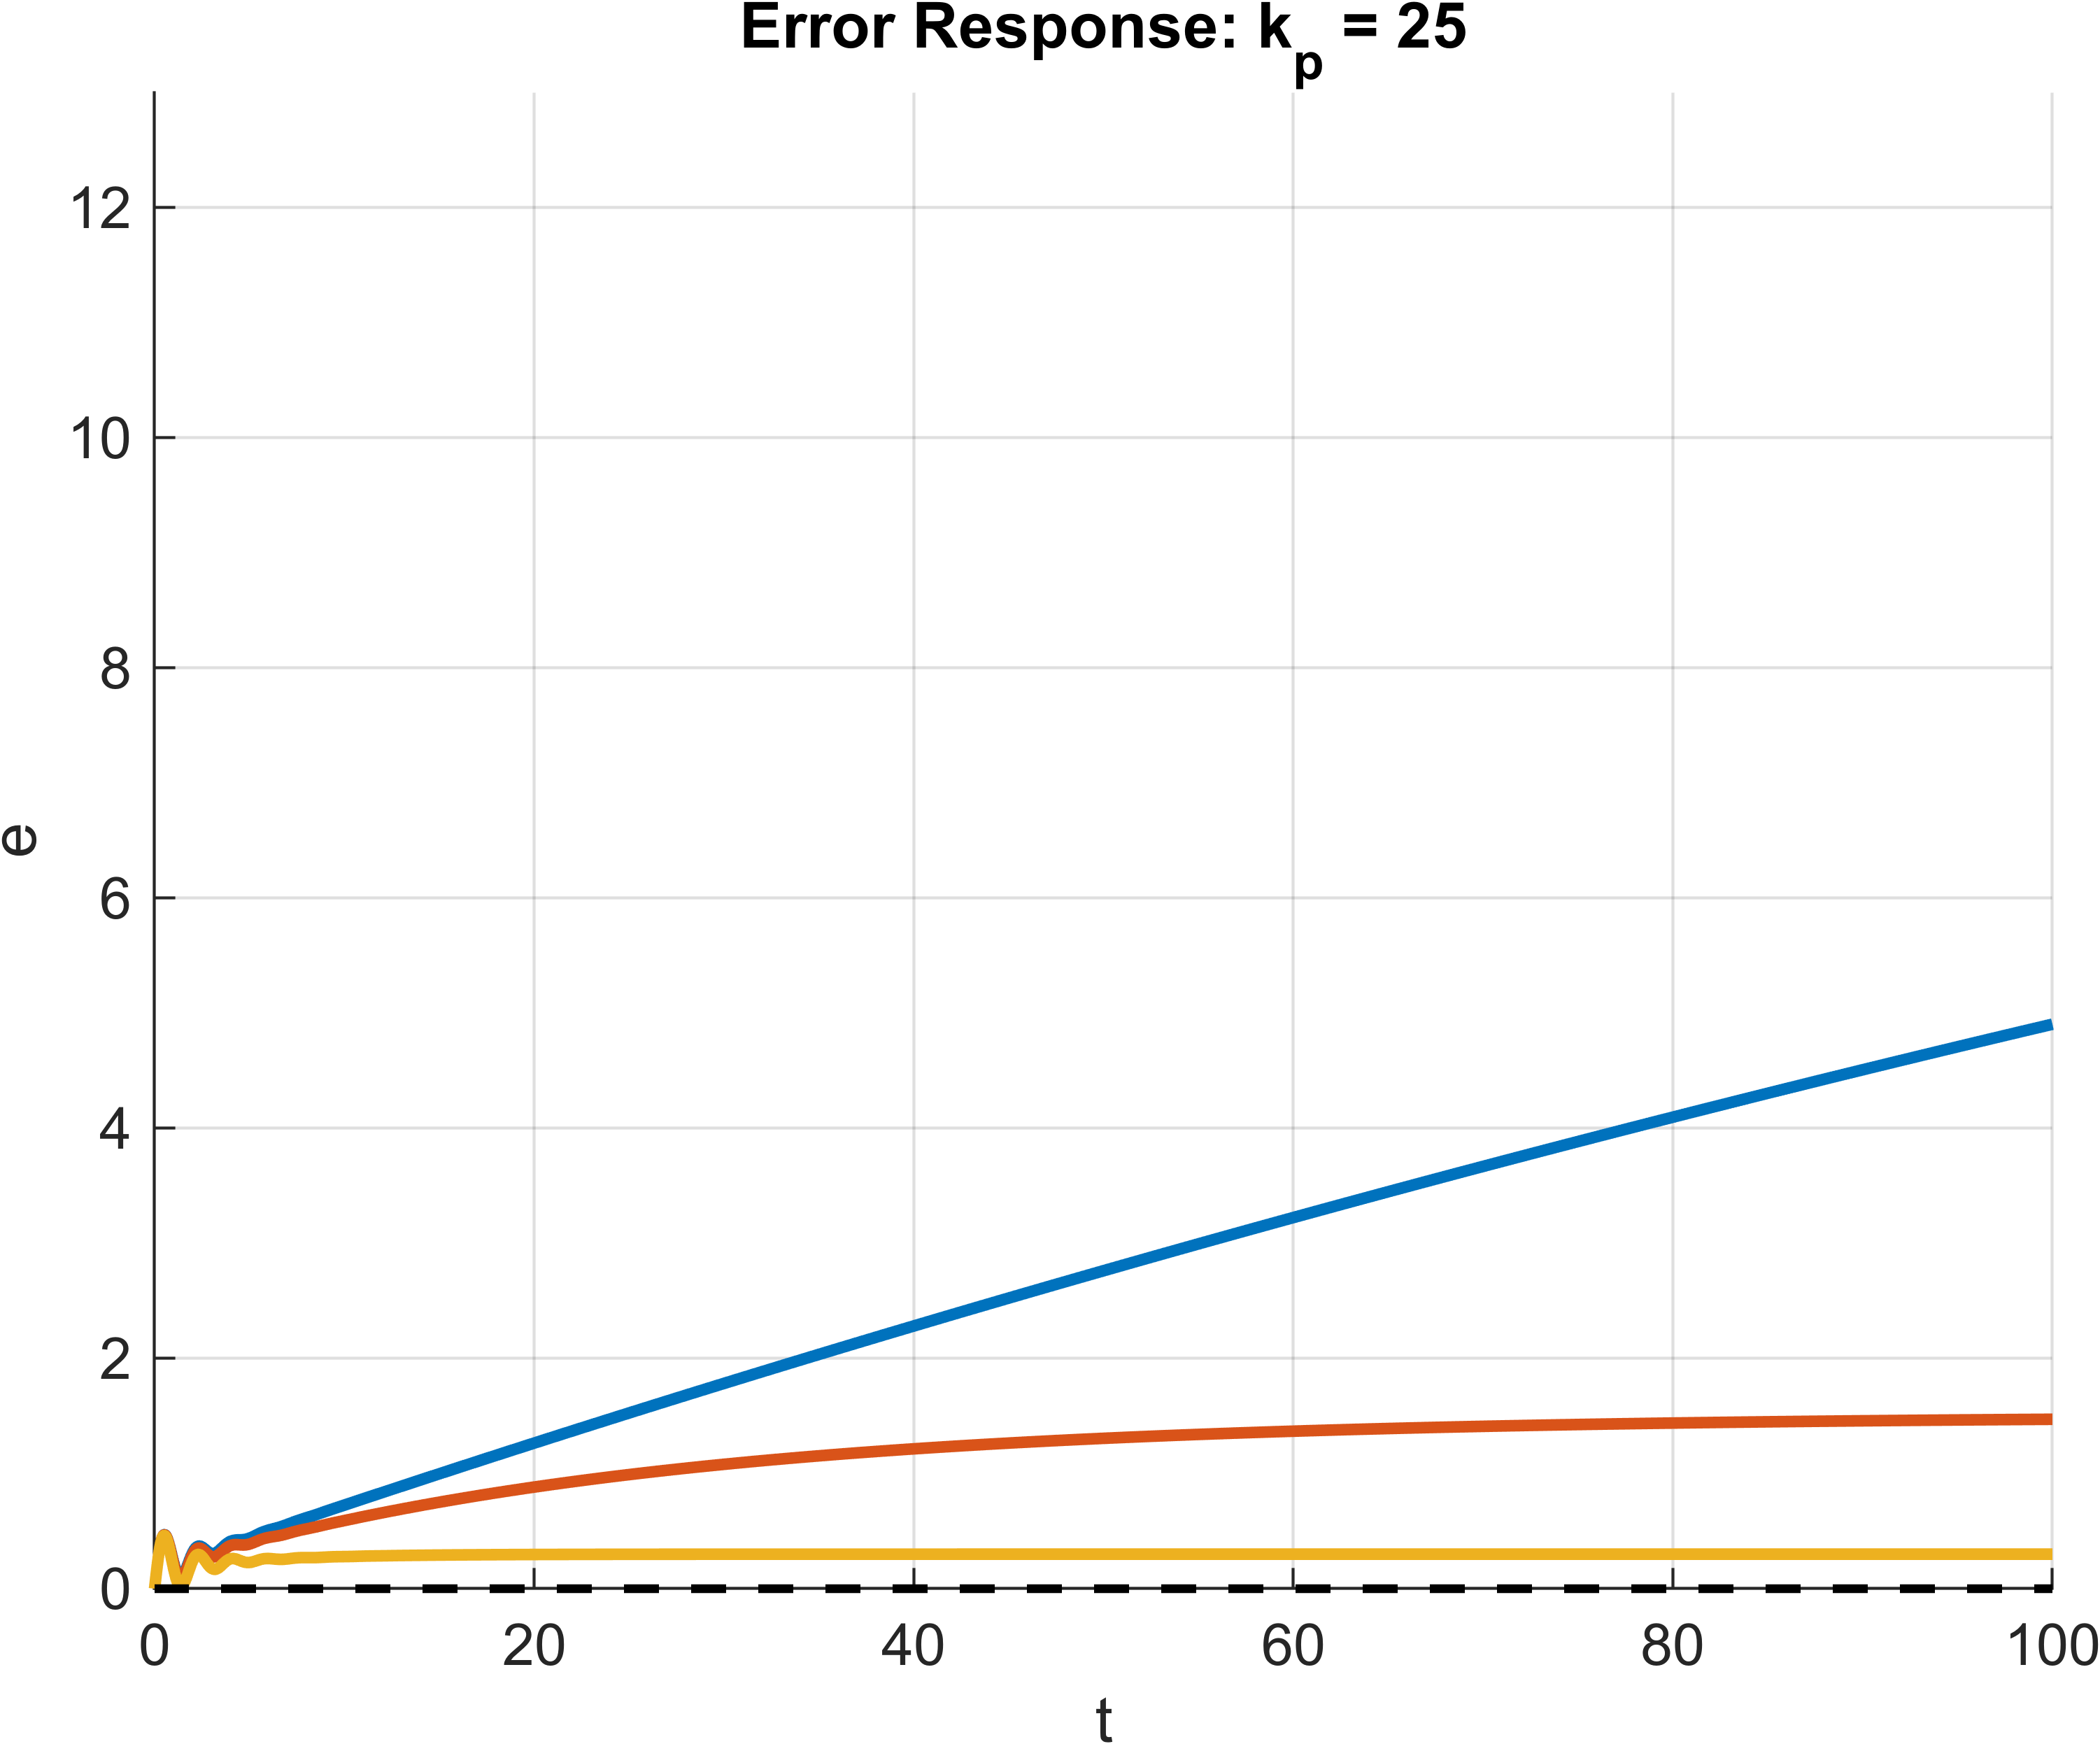
\includegraphics[width=1\textwidth, trim={1cm 0cm 1cm 0cm}]{../images/input_2_kp_25_error.png}
    \end{minipage}
    \caption{Графики $y(t)$ и $e(t)$ при $g(t) = 1.5t$ и $k_p = 25$}
\end{figure}

Аналитически определим предельное значение ошибки $e$ для каждой пары $k_p$ и $k_i$:
\[
    W_{g\to e} = \frac{1}{1 + (k_p+\frac{k_i}{s}) W(s)}
    = \frac{s}{s + (k_p+\frac{k_i}{s}) \frac{1}{2s^2 + 3s + 1}}
    = \frac{2s^3 + 3s^2 + s}{2s^3 + 3s^2 + s + k_p s + k_i}
\]
\[
    e_{\text{уст}} = \lim_{t \to \infty} e(t)
    = \lim_{s \to 0} s E(s)
    = \lim_{s \to 0} s W_{g\to e} G(s) =
\]\[
    = \lim_{s \to 0} s \frac{2s^3 + 3s^2 + s}{2s^3 + 3s^2 + s + k_p s + k_i} \frac{1.5}{s^2}
    = \frac{1.5}{k_i}
\]
\[
    k_i = 0.1, \, k_p = 5,\, 10,\, 25: e_{\text{уст}} = 15
\]
\[
    k_i = 1, \, k_p = 5,\, 10,\, 25: e_{\text{уст}} = 1.5
\]
\[
    k_i = 5, \, k_p = 5,\, 10,\, 25: e_{\text{уст}} = 0.3
\]

Из графиков и аналитических расчетов видно, что ПИ-регулятор 
обеспечивает постоянную установившуюся ошибку. При этом она 
зависит от $k_i$ и не зависит от $k_p$.

\section{Режим слежения за гармоническим сигналом при $g(t) = a\sin(\omega t)$}
Выполним моделирование:
\begin{figure}[H]
    \centering
    \begin{minipage}{0.45\textwidth}
        \centering
        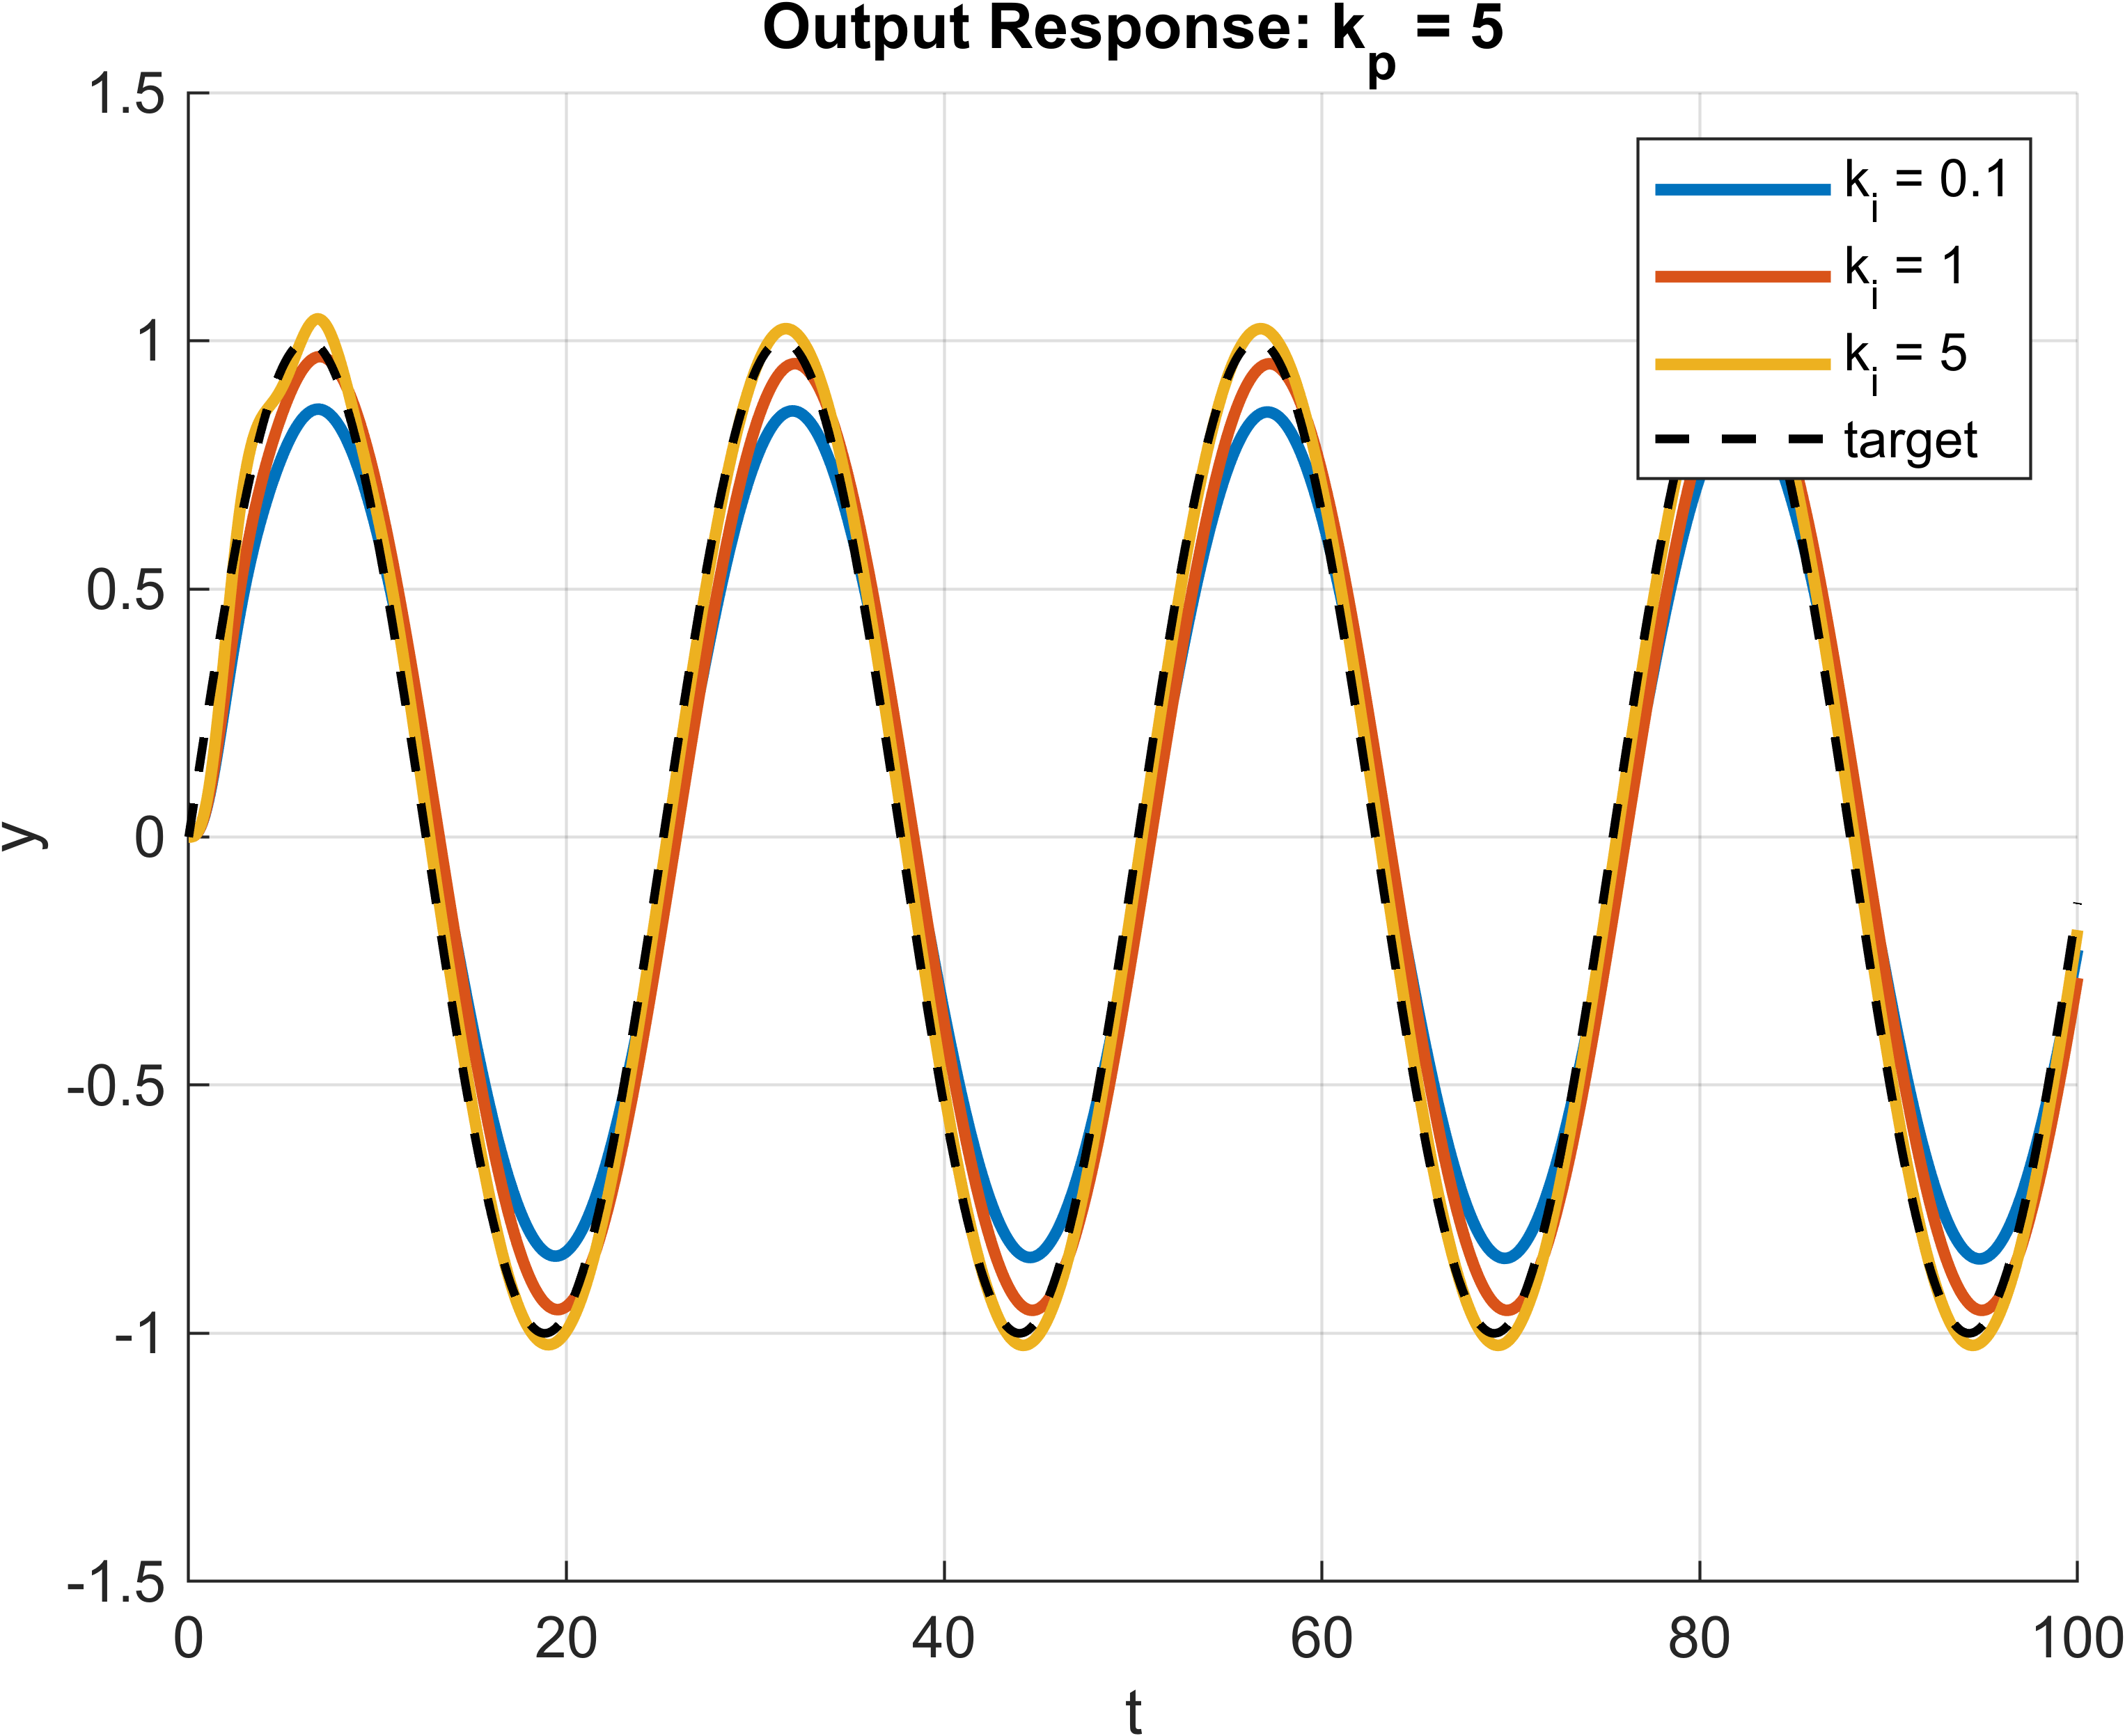
\includegraphics[width=1\textwidth, trim={1cm 0cm 1cm 0cm}]{../images/input_4_kp_5_output.png}
    \end{minipage}
    \hfill
    \begin{minipage}{0.45\textwidth}
        \centering
        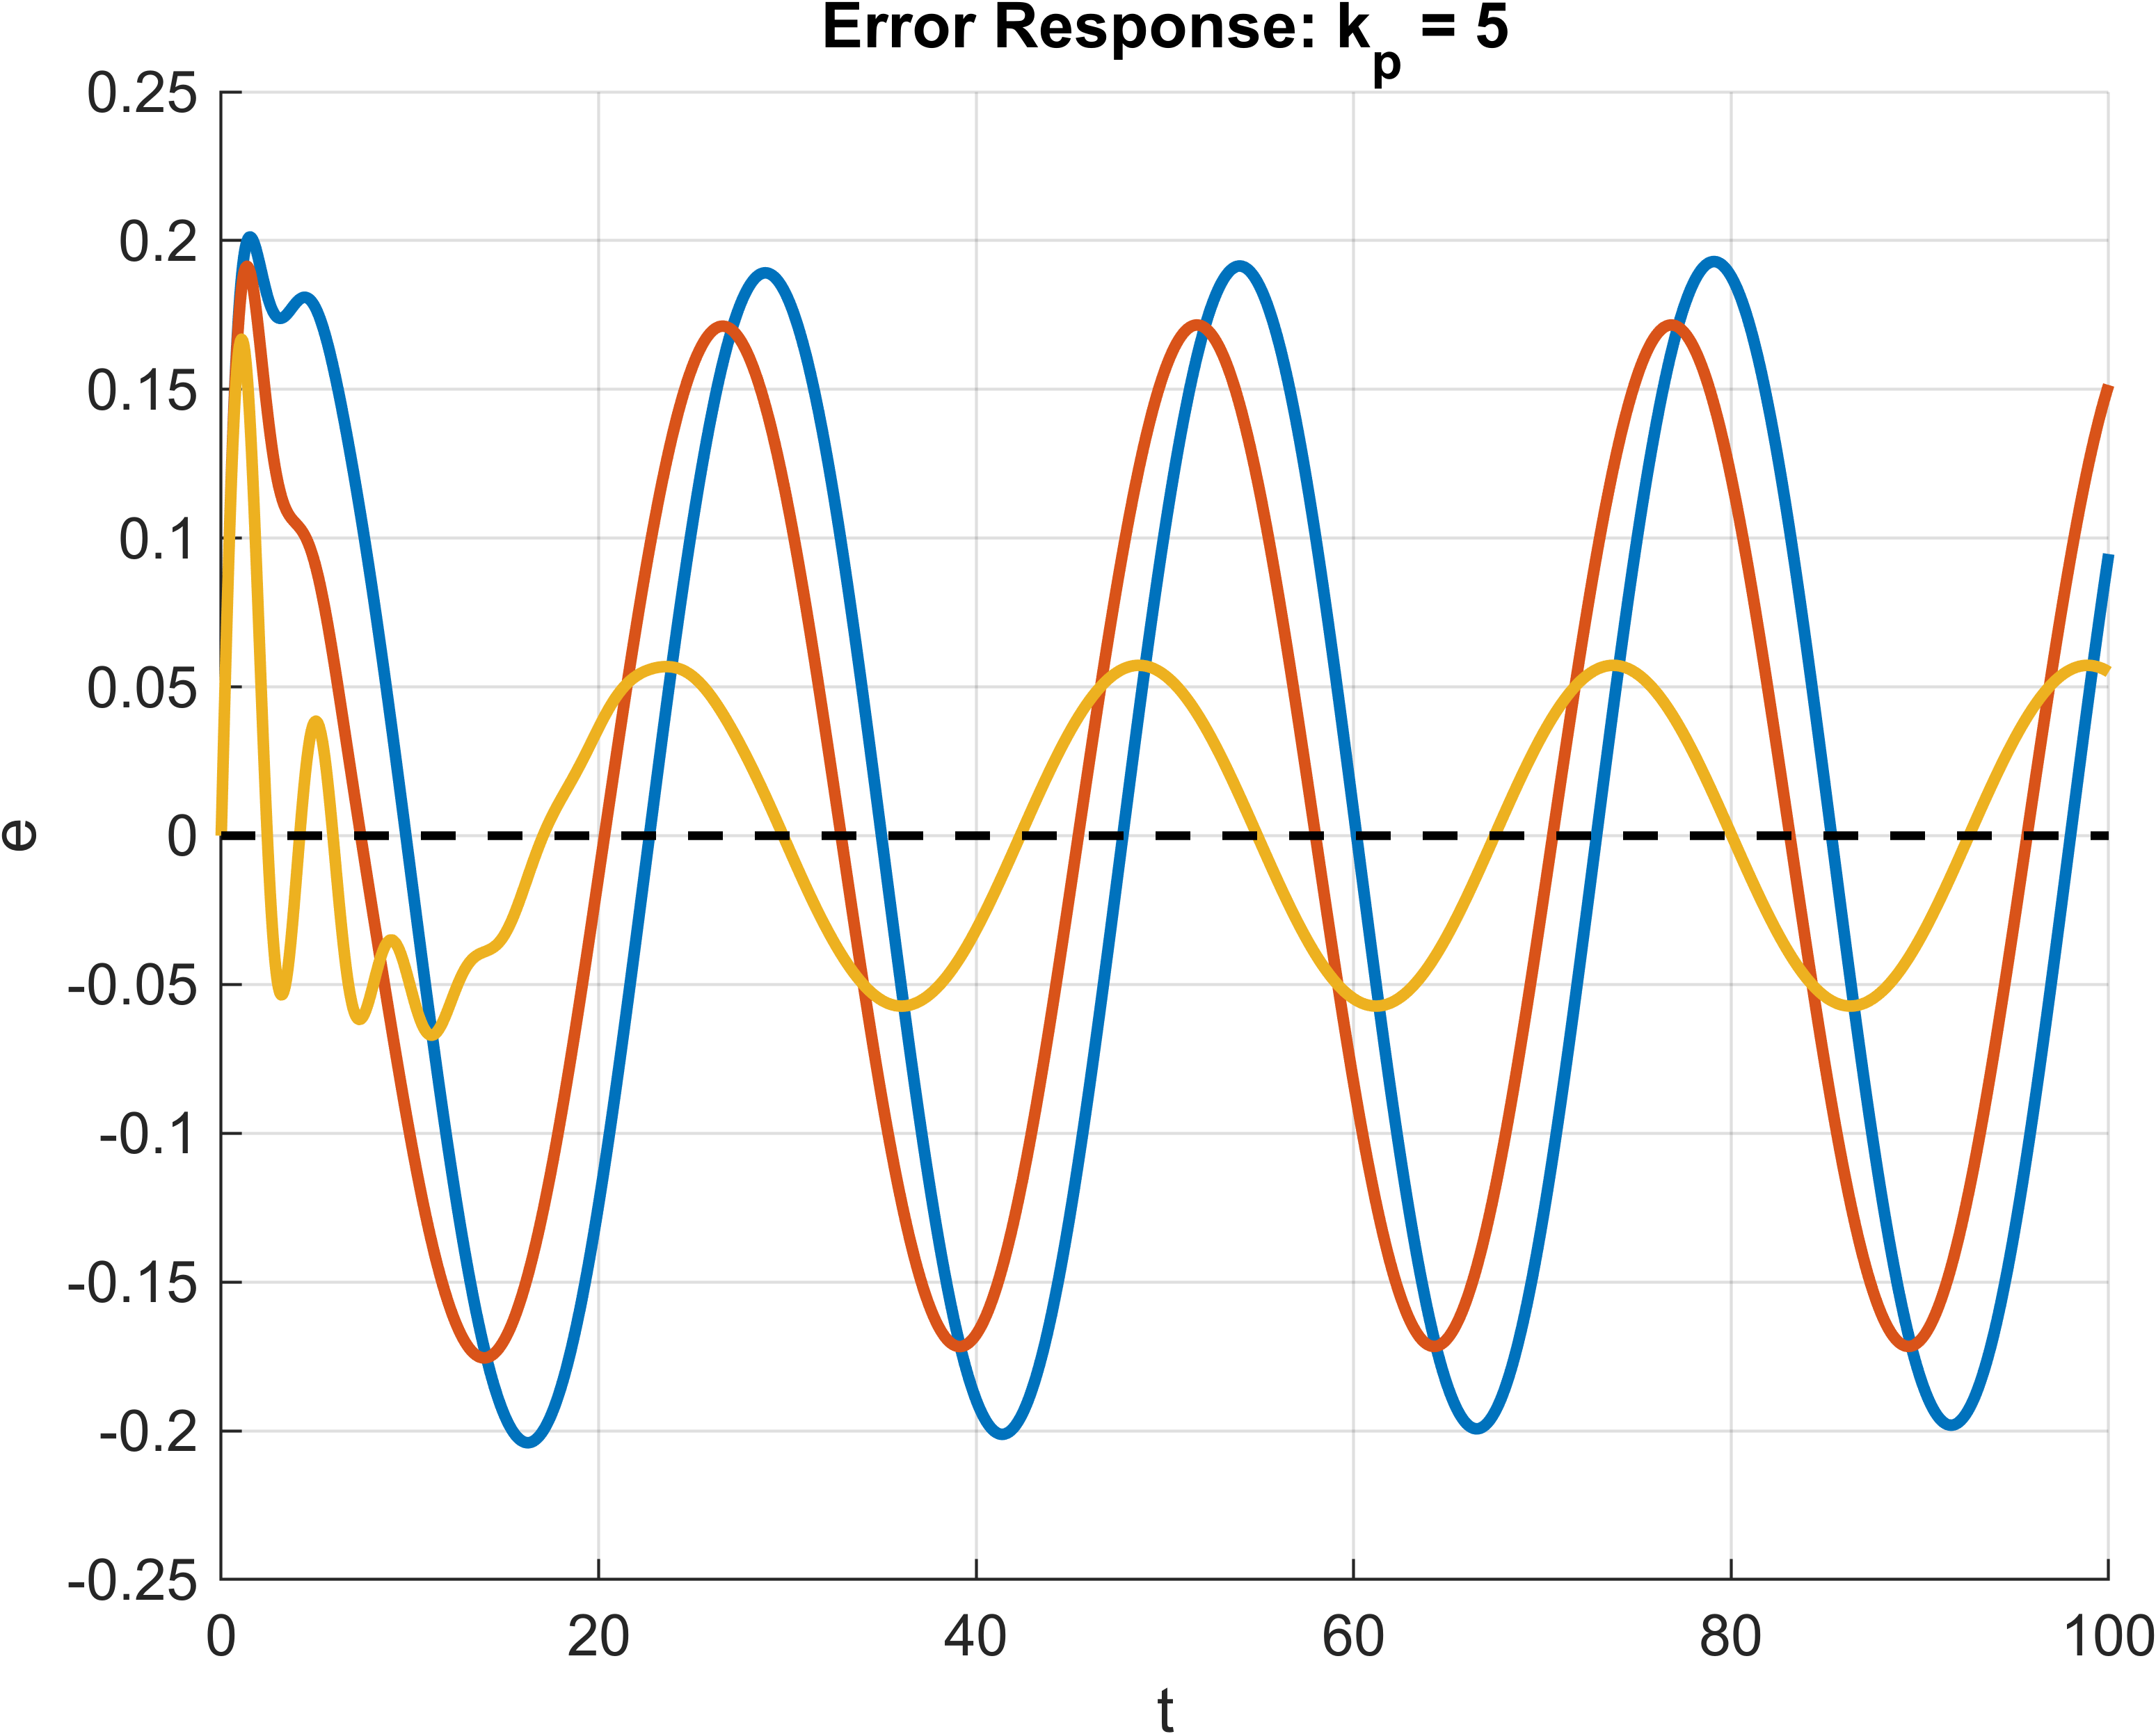
\includegraphics[width=1\textwidth, trim={1cm 0cm 1cm 0cm}]{../images/input_4_kp_5_error.png}
    \end{minipage}
    \caption{Графики $y(t)$ и $e(t)$ при $g(t) = \sin(0.25t)$ и $k_p = 5$}
\end{figure}
\begin{figure}[H]
    \centering
    \begin{minipage}{0.45\textwidth}
        \centering
        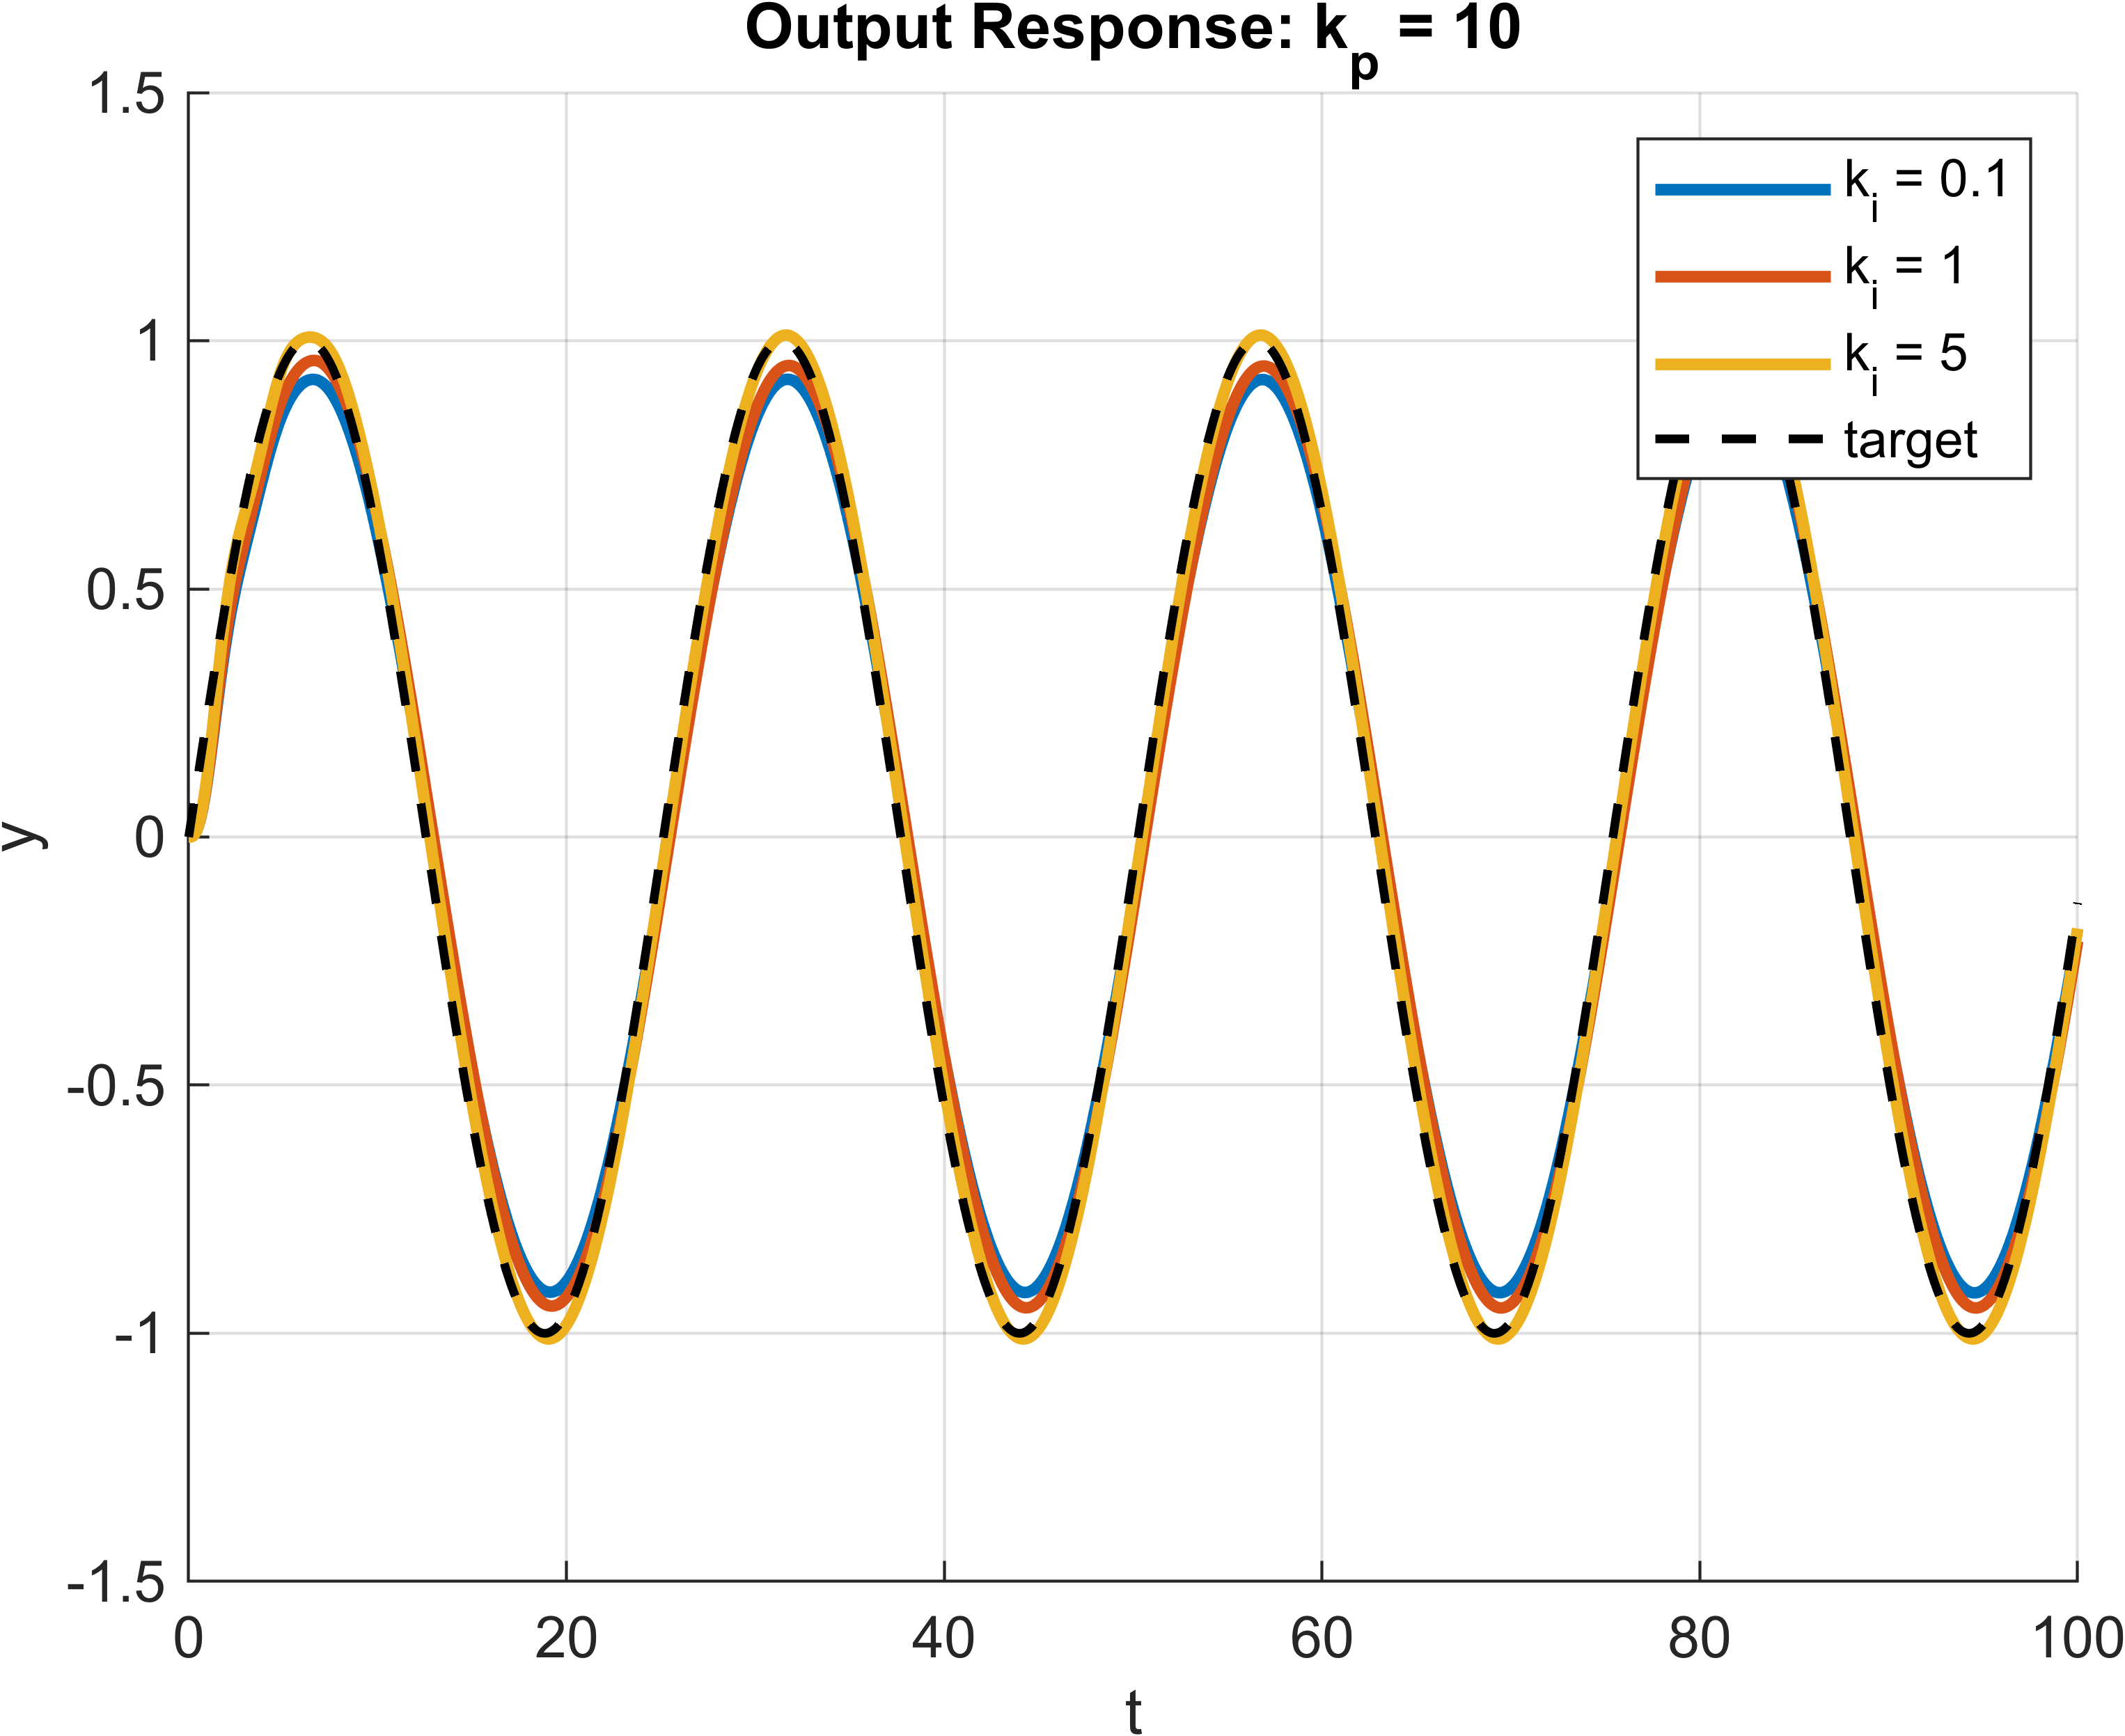
\includegraphics[width=1\textwidth, trim={1cm 0cm 1cm 0cm}]{../images/input_4_kp_10_output.png}
    \end{minipage}
    \hfill
    \begin{minipage}{0.45\textwidth}
        \centering
        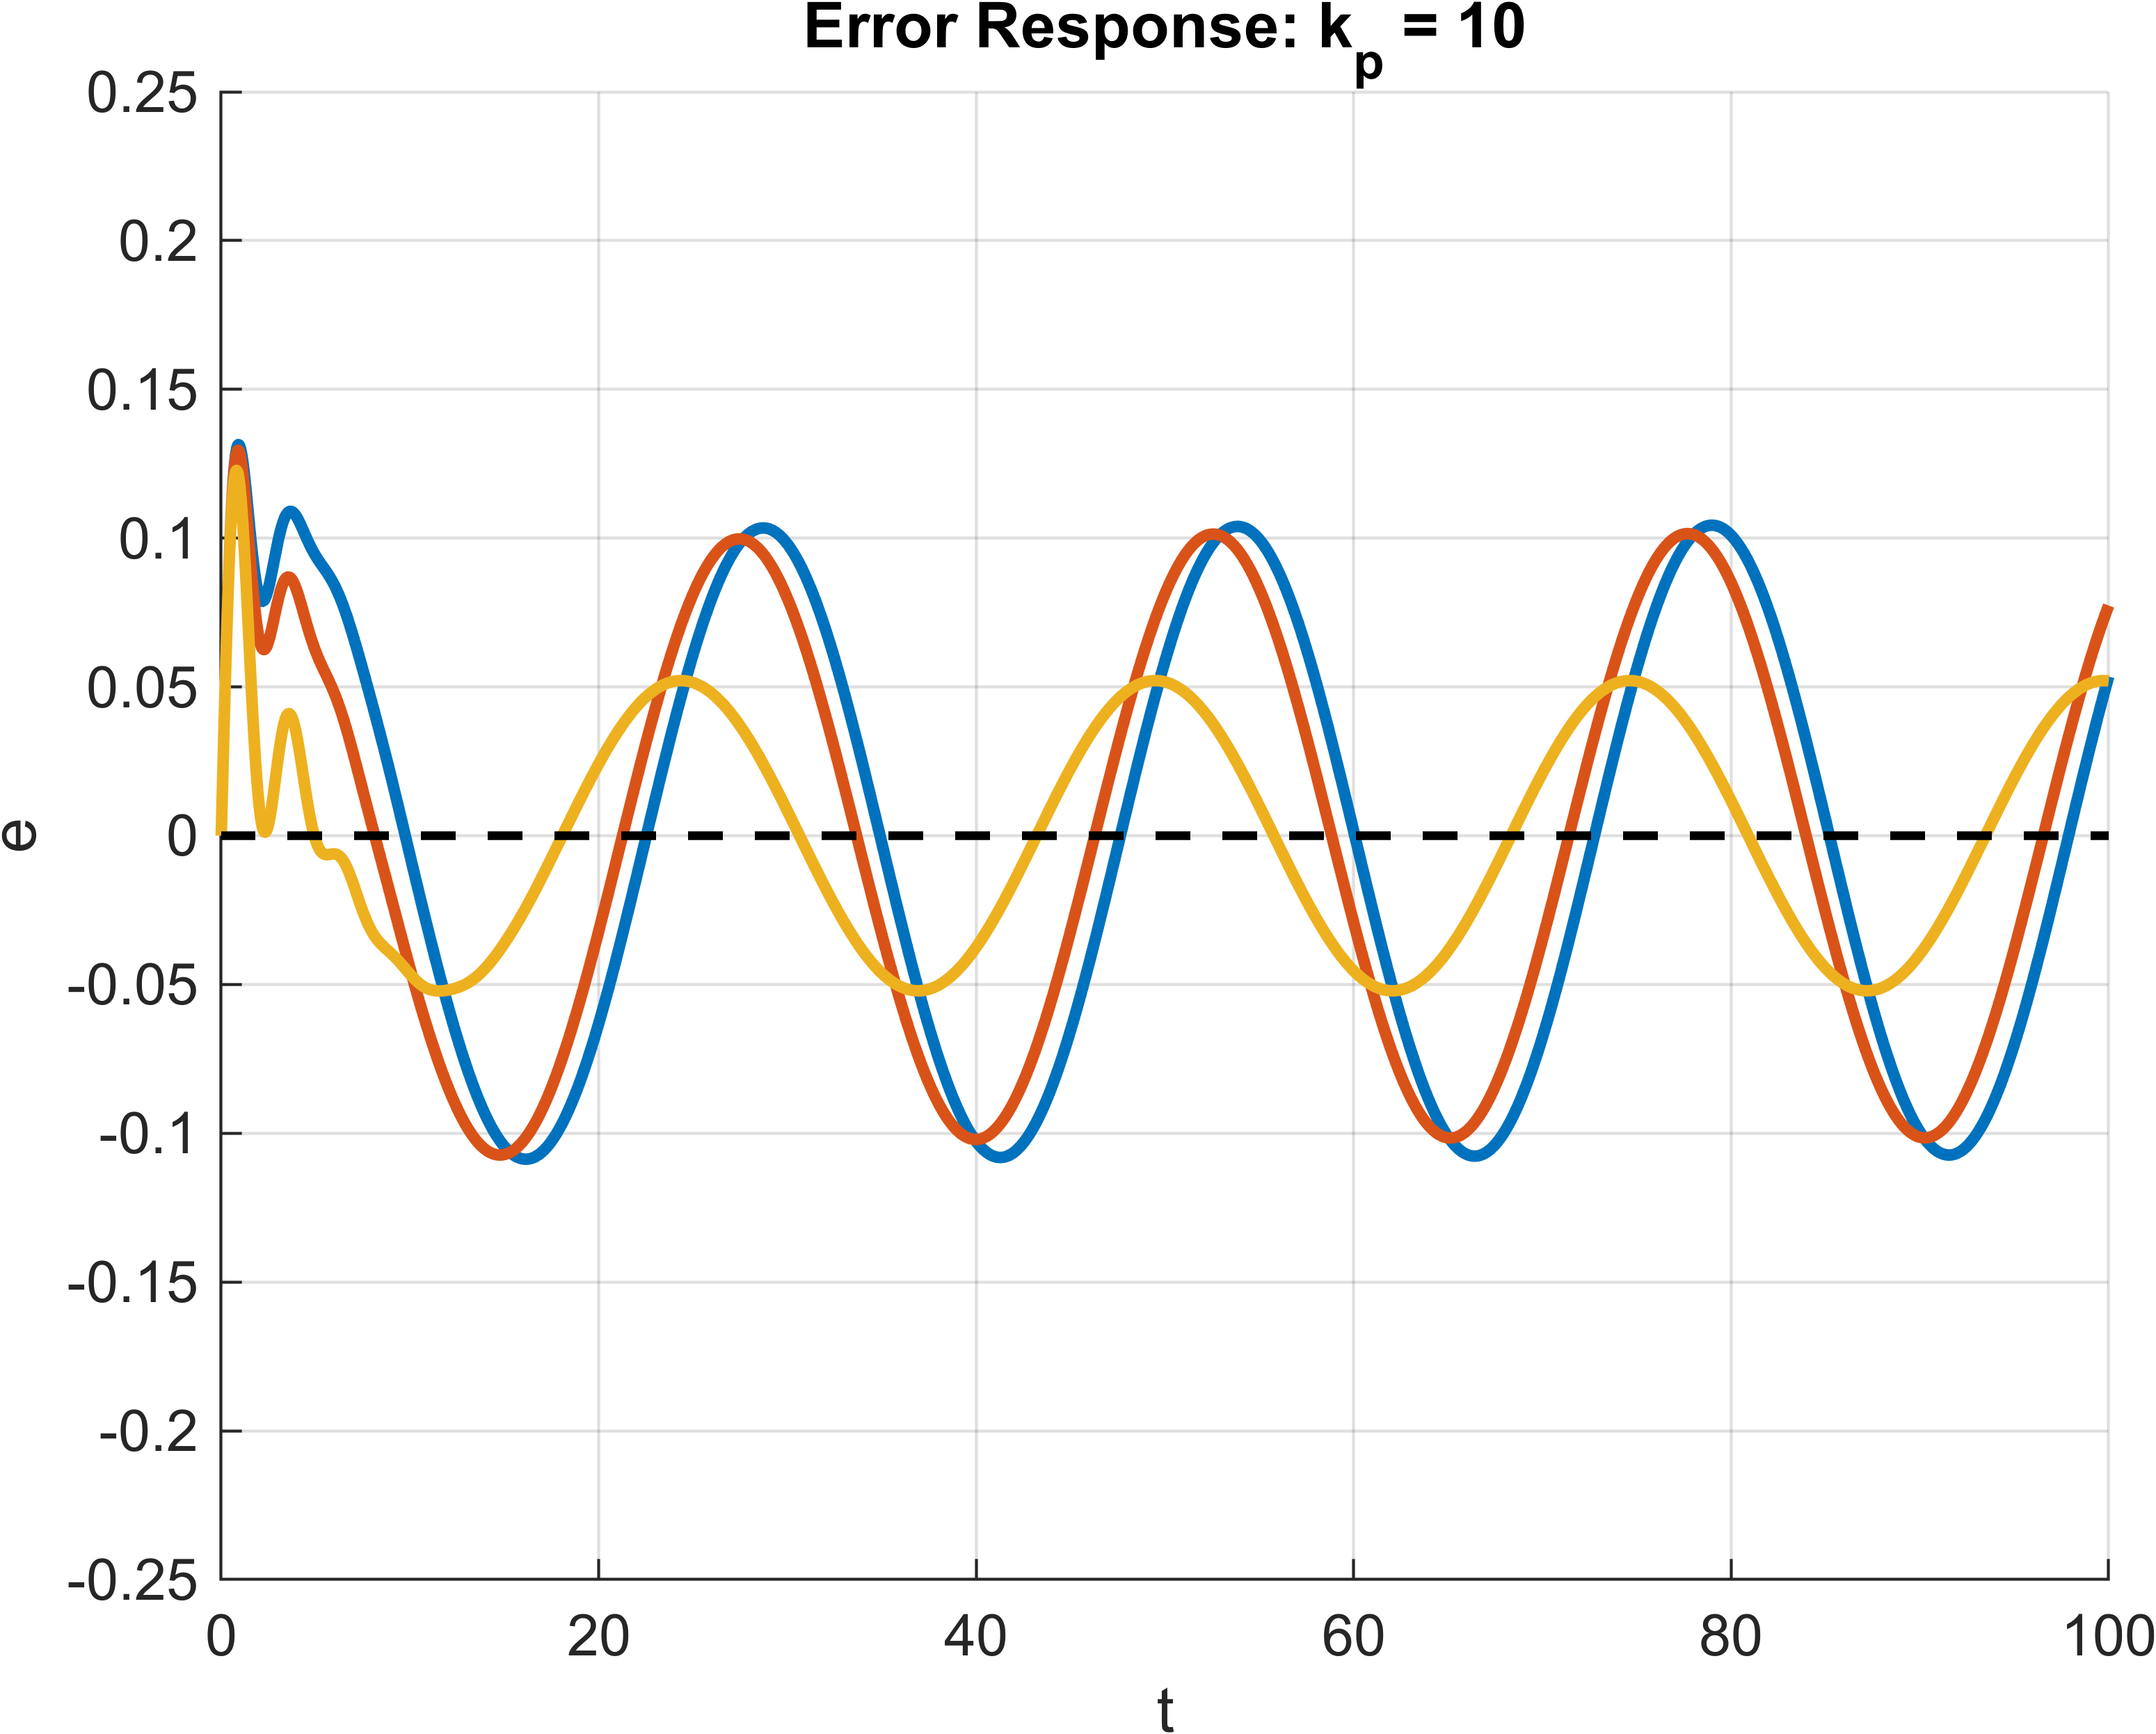
\includegraphics[width=1\textwidth, trim={1cm 0cm 1cm 0cm}]{../images/input_4_kp_10_error.png}
    \end{minipage}
    \caption{Графики $y(t)$ и $e(t)$ при $g(t) = \sin(0.25t)$ и $k_p = 10$}
\end{figure}
\begin{figure}[H]
    \centering
    \begin{minipage}{0.45\textwidth}
        \centering
        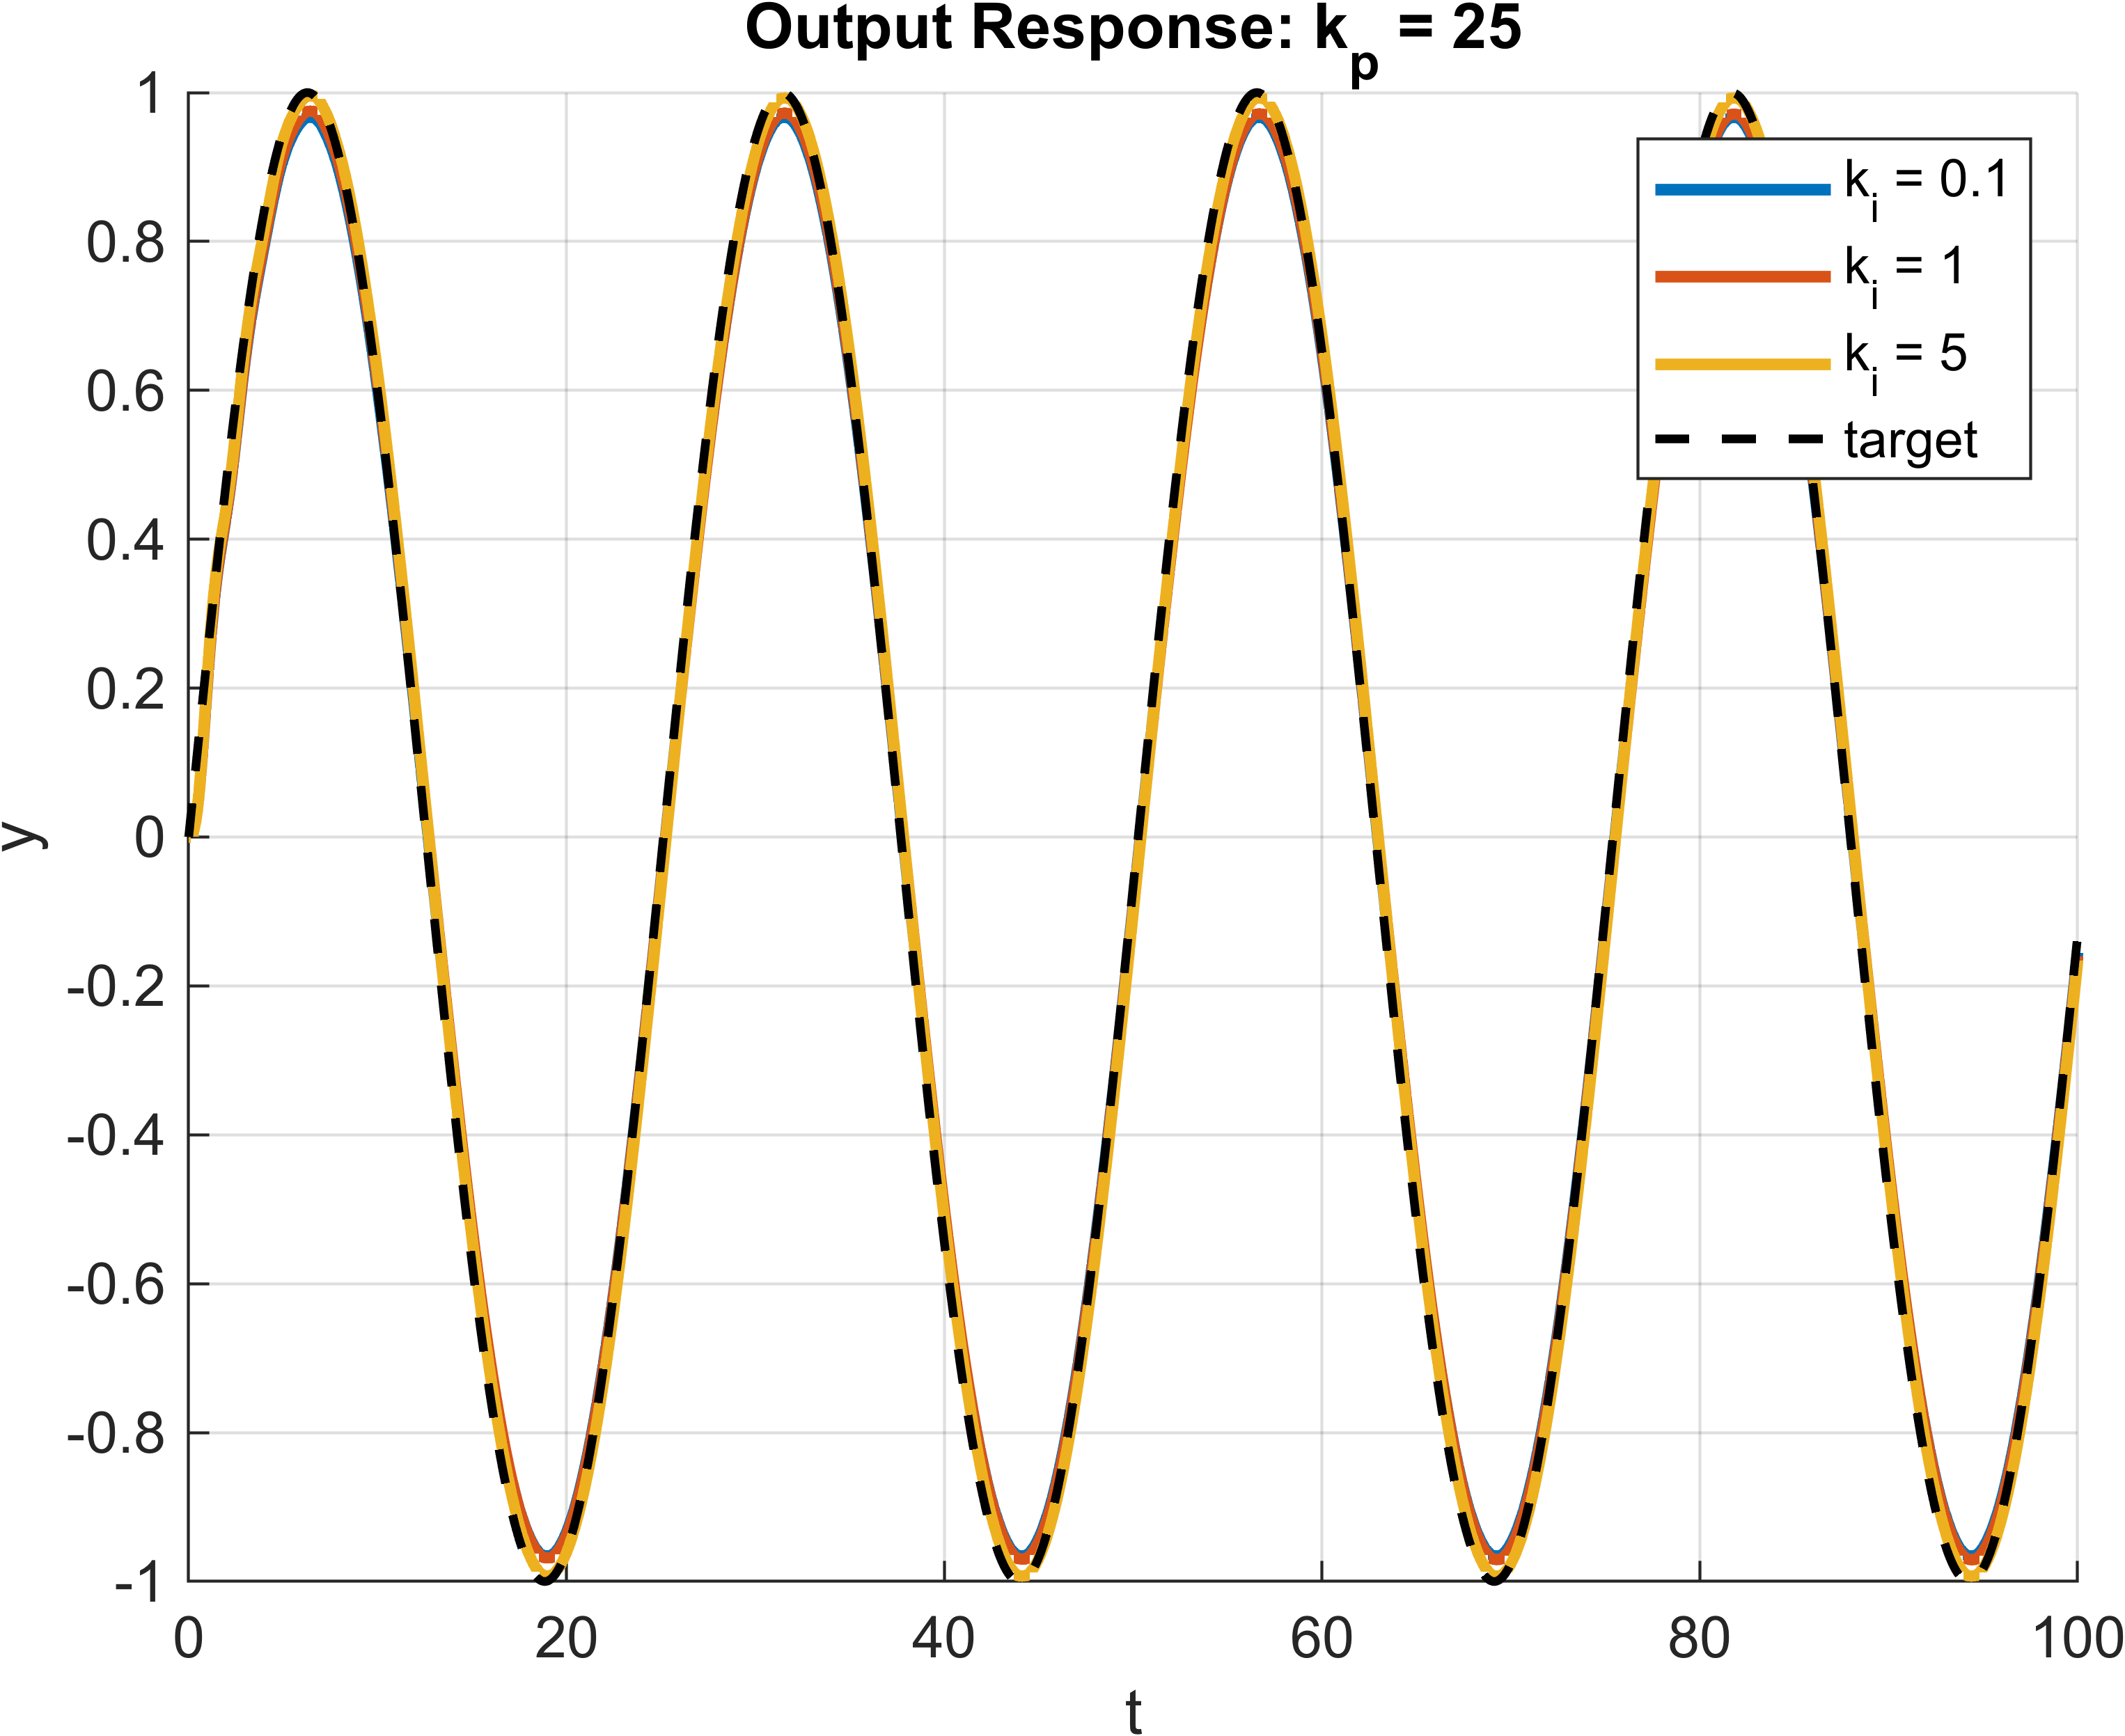
\includegraphics[width=1\textwidth, trim={1cm 0cm 1cm 0cm}]{../images/input_4_kp_25_output.png}
    \end{minipage}
    \hfill
    \begin{minipage}{0.45\textwidth}
        \centering
        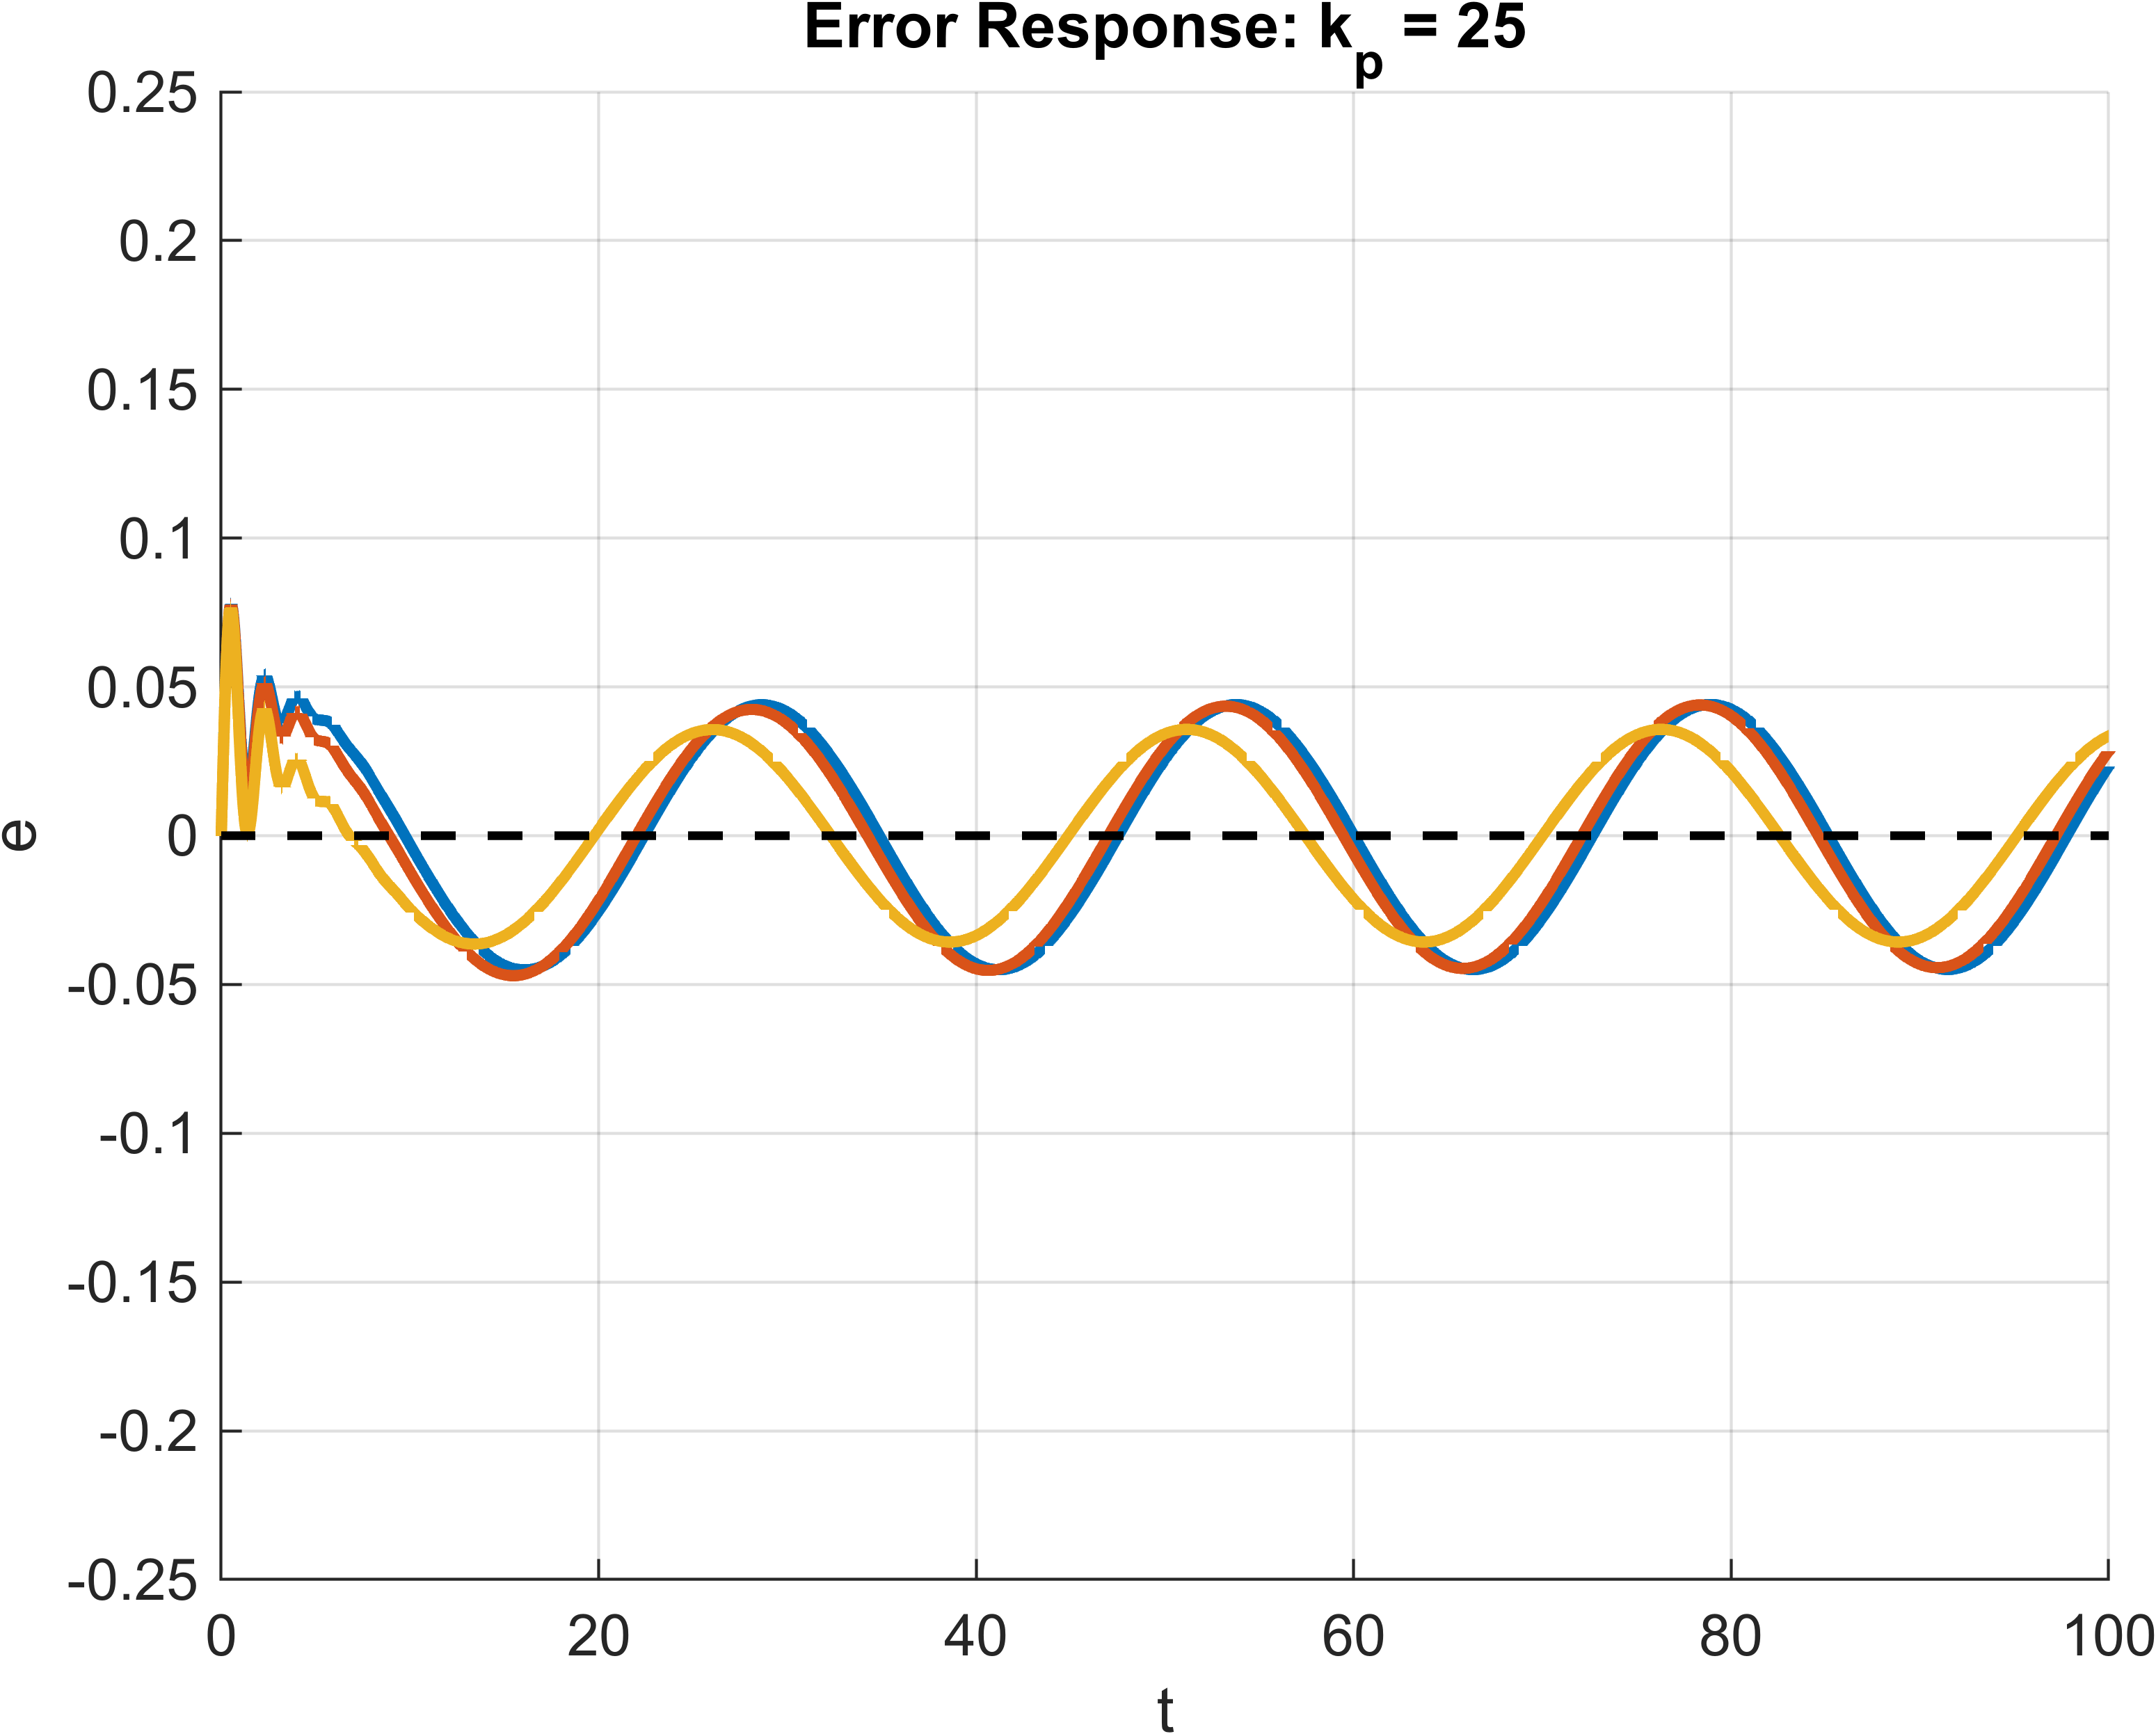
\includegraphics[width=1\textwidth, trim={1cm 0cm 1cm 0cm}]{../images/input_4_kp_25_error.png}
    \end{minipage}
    \caption{Графики $y(t)$ и $e(t)$ при $g(t) = \sin(0.25t)$ и $k_p = 25$}
\end{figure}

Как видно из графиков, ПИ-регулятор не может обеспечить 
слежение за гармоническим сигналом. Ошибка имеет гармонический характер.
Увеличение коэффициентов $k_p$ и $k_i$ уменьшает амплитуду ошибки.
\endinput
